% !TEX root = ./notes_template.tex
%%%%%%%%%%%%%%%%%%%%%%%%%%%%%%%%%%%%%%%%%%%%%%%%%%
%%%%%%%%%%%%%%%%%%%%% preamble %%%%%%%%%%%%%%%%%%%
%%%%%%%%%%%%%%%%%%%%%%%%%%%%%%%%%%%%%%%%%%%%%%%%%%
\documentclass[11pt,twoside]{book}


\usepackage{luatex85}


\usepackage{ctex}
\renewcommand{\contentsname}{目录}
\usepackage{fontspec}
\usepackage{xeCJK}
\setCJKmainfont{LXGW WenKai Mono}
\linespread{1.5}


\usepackage{xeCJKfntef}
\xeCJKsetup{underdot/symbol={\normalfont^^b7}}
\newcommand{\dotemph}[1]{\CJKunderdot{#1}}


\usepackage[multiple]{footmisc}

%\renewcommand{\baselinestretch}{1.05}
\usepackage{amsmath,amsthm,amssymb,mathrsfs,amsfonts,dsfont}
\usepackage{epsfig,graphicx}
\usepackage{tabularx}
\usepackage{blkarray}
\usepackage{slashed}
\usepackage{color}
\usepackage{listings}
\usepackage{caption}
% \usepackage{fullpage}
\usepackage{lipsum} % provides dummy text for testing
\usepackage[toc,title,titletoc,header]{appendix}
\usepackage{minitoc}
\usepackage{color}
\usepackage{multicol} % two-col ToC
\usepackage{bm}
\usepackage{imakeidx} % before hyperref
\usepackage{hyperref}
% link colors settings
\hypersetup{
    colorlinks=true,
    citecolor=magenta,
    linkcolor=magenta,
    filecolor=green,      
    urlcolor=cyan,
    % hypertexnames=false,
}
\usepackage[capitalise]{cleveref}
\usepackage{subcaption}
\usepackage{enumitem}
\usepackage{mathtools}
\usepackage{physics}
\usepackage[linesnumbered,ruled,vlined,algosection]{algorithm2e}
\SetCommentSty{textsf}
\usepackage{epigraph}
\epigraphwidth=1.0\linewidth
\epigraphrule=0pt

% adjust margin
\usepackage[margin=2.3cm]{geometry}
\headheight13.6pt

%%%%%%%%%%%%%%%% thmtools %%%%%%%%%%%%%%%%%%%%%
\usepackage{thmtools}
\declaretheorem[numberwithin=chapter]{theorem}
\declaretheorem[numberwithin=chapter]{axiom}
\declaretheorem[numberwithin=chapter]{lemma}
\declaretheorem[numberwithin=chapter]{proposition}
\declaretheorem[numberwithin=chapter]{claim}
\declaretheorem[numberwithin=chapter]{conjecture}
\declaretheorem[sibling=theorem]{corollary}
\declaretheorem[numberwithin=chapter, style=definition]{definition}
\declaretheorem[numberwithin=chapter, style=definition]{problem}
\declaretheorem[numberwithin=chapter, style=definition]{example}
\declaretheorem[numberwithin=chapter, style=definition]{exercise}
\declaretheorem[numberwithin=chapter, style=definition]{observation}
\declaretheorem[numberwithin=chapter, style=definition]{fact}
\declaretheorem[numberwithin=chapter, style=definition]{construction}
\declaretheorem[numberwithin=chapter, style=definition]{remark}
\declaretheorem[numberwithin=chapter, style=remark]{question}
%%%%%%%%%%%%%%%% thmtools %%%%%%%%%%%%%%%%%%%%%
\usepackage{changepage}
\newenvironment{solution}
    {\renewcommand\qedsymbol{$\square$}\color{blue}\begin{adjustwidth}{0em}{2em}\begin{proof}[\textit Solution.~]}
    {\end{proof}\end{adjustwidth}}

%%%%%%%%%%%%%%%% index %%%%%%%%%%%%%%%%%%%%%
\begin{filecontents}{index.ist}
% https://tex.stackexchange.com/questions/65247/index-with-an-initial-letter-of-the-group
headings_flag 1
heading_prefix "{\\centering\\large \\textbf{"
heading_suffix "}}\\nopagebreak\n"
delim_0 "\\nobreak\\dotfill"
\end{filecontents}
\newcommand{\myindex}[1]{\index{#1} \emph{#1}}
\makeindex[columns=3, intoc, title=Alphabetical Index, options= -s index.ist]
%%%%%%%%%%%%%%%% index %%%%%%%%%%%%%%%%%%%%%

%%%%%%%%%%%%%%%% ToC %%%%%%%%%%%%%%%%%%%%%
% Link Chapter title to ToC: https://tex.stackexchange.com/questions/32495/linking-the-section-text-to-the-toc
\usepackage[explicit]{titlesec}
\titleformat{\chapter}[display]
  {\normalfont\huge\bfseries}{\chaptertitlename\ {\thechapter}}{20pt}{\hyperlink{chap-\thechapter}{\Huge#1}
\addtocontents{toc}{\protect\hypertarget{chap-\thechapter}{}}}
\titleformat{name=\chapter,numberless}
  {\normalfont\huge\bfseries}{}{-20pt}{\Huge#1}

\titleformat{\subsubsection}[runin]
  {\normalfont\large\bfseries}{}{}{#1}[]


%%%%%%%%%%%%%%%%%%% fancyhdr %%%%%%%%%%%%%%%%%
\usepackage{fancyhdr}
\pagestyle{fancy} % enable fancy page style
\renewcommand{\headrulewidth}{0.0pt} % comment if you want the rule
\fancyhf{} % clear header and footer
\fancyhead[lo,le]{\leftmark}
\fancyhead[re,ro]{\rightmark}
\fancyfoot[CE,CO]{\hyperref[toc-contents]{\thepage}}

% https://tex.stackexchange.com/questions/550520/making-each-page-number-link-back-to-beginning-of-chapter-or-section
\makeatletter
\def\chaptermark#1{\markboth{\protect\hyper@linkstart{link}{\@currentHref}{Chapter \thechapter ~ #1}\protect\hyper@linkend}{}}
\def\sectionmark#1{\markright{\protect\hyper@linkstart{link}{\@currentHref}{\thesection ~ #1}\protect\hyper@linkend}}
\makeatother
%%%%%%%%%%%%%%%%%%% fancyhdr %%%%%%%%%%%%%%%%%


%%%%%%%%%%%%%%%%%%% biblatex %%%%%%%%%%%%%%%%%
\usepackage[doi=false,url=false,isbn=false,style=alphabetic,backend=biber,backref=true, minalphanames=3]{biblatex}

\DefineBibliographyStrings{english}{
  backrefpage={Cited on page},
  backrefpages={Cited on pages}
}

\addbibresource{bib.bib}

\newbibmacro{string+doiurlisbn}[1]{%
  \iffieldundef{doi}{%
    \iffieldundef{url}{%
      \iffieldundef{isbn}{%
        \iffieldundef{issn}{%
          #1%
        }{%
          \href{http://books.google.com/books?vid=ISSN\thefield{issn}}{#1}%
        }%
      }{%
        \href{http://books.google.com/books?vid=ISBN\thefield{isbn}}{#1}%
      }%
    }{%
      \href{\thefield{url}}{#1}%
    }%
  }{%
    \href{http://dx.doi.org/\thefield{doi}}{#1}%
  }%
}

% https://tex.stackexchange.com/questions/94089/remove-quotes-from-inbook-reference-title-with-biblatex
\DeclareFieldFormat[article,incollection,inproceedings,book,misc]{title}{\usebibmacro{string+doiurlisbn}{\mkbibemph{#1}}}
% https://tex.stackexchange.com/questions/454672/biblatex-journal-name-non-italic
\DeclareFieldFormat{journaltitle}{#1\isdot}
\DeclareFieldFormat{booktitle}{#1\isdot}
% https://tex.stackexchange.com/questions/10682/suppress-in-biblatex
\renewbibmacro{in:}{}
% add video field: https://tex.stackexchange.com/questions/111846/biblatex-2-custom-fields-only-one-is-working
\DeclareSourcemap{
    \maps[datatype=bibtex]{
      \map{
        \step[fieldsource=video]
        \step[fieldset=usera,origfieldval]
    }
  }
}
\DeclareFieldFormat{usera}{\href{#1}{\textsc{Online video}}}
\AtEveryBibitem{
    \csappto{blx@bbx@\thefield{entrytype}}{% put at end of entry
        \iffieldundef{usera}{}{\space \printfield{usera}}
    }
}
%%%%%%%%%%%%%%%%%%% biblatex %%%%%%%%%%%%%%%%%

%%%%%%%%%%%%%%%%%%%%% glossaries %%%%%%%%%%%%%%%%%
% !TEX root = ./notes_template.tex
% \usepackage[style=super]{glossaries}
% https://www.overleaf.com/learn/latex/Glossaries
\usepackage[style=super,toc,acronym]{glossaries}
\setlength{\glsdescwidth}{1\linewidth}
\makeglossaries

\renewcommand\glossaryname{List of Abbreviations and Symbols}

\newglossaryentry{Q2}{name={$Q_2(f)$},
%sort=Q2,
description={Two-side (bounded) error quantum query complexity}}

\newglossaryentry{real_number}{name={$\mathbb{R}$},description={Real number}}

% \newglossaryentry{gcd}{name={gcd},description={greatest common divisor}}

\newacronym{gcd}{GCD}{Greatest Common Divisor}


\newglossaryentry{svm}{name={SVM},description={Support Vector Machine}}

\newglossaryentry{gd}{name={GD},description={Gradient Descent}}

\newglossaryentry{qft}{name={QFT},description={Quantum Field Theory}}

\newglossaryentry{qm}{name={QM},description={Quantum Mechanics}}

\newglossaryentry{v}{name={$\vec{v}$},description={a vector}}

% physics
\newglossaryentry{hamiltonian}{name={$\hat{H}$},description={Hamiltonian}}

\newglossaryentry{lagrangian}{name={$L$},description={Lagrangian}}
%%%%%%%%%%%%%%%%%%%%% glossaries %%%%%%%%%%%%%%%%%

%%%%%%%%%%%%%%%%%%%%% glossaries-extra %%%%%%%%%%%%%%%%%
% \usepackage[record,abbreviations,symbols,stylemods={list,tree,mcols}]{glossaries-extra}
%%%%%%%%%%%%%%%%%%%%% glossaries-extra %%%%%%%%%%%%%%%%%


% !TEX root = ./notes_template.tex

%%%%%%%%%%%%%%%%%%%%%%%%%%%%%%%%%%%%
%%%%%%%%%%%%%%%%%%%%%%%%%%%%%%%%%%%%
% math
\let\iff\relax
\newcommand{\iff}{\text{ iff }}
\newcommand{\OPT}{\textup{OPT}}

% physics
\newcommand{\acreation}{a^\dagger}



%%%%%%%%%%%%%%%%%%%%%%%%%%%%%%%%%%%%%%%%%%%%%%%%%%
%%%%%%%%%%%%%%%% begin of document %%%%%%%%%%%%%%%
%%%%%%%%%%%%%%%%%%%%%%%%%%%%%%%%%%%%%%%%%%%%%%%%%%

\begin{document}

\title{\bf \huge 理解 PLONK}
\author{安比实验室}
\date{\today}
\maketitle
\setcounter{tocdepth}{2}
\setcounter{minitocdepth}{1} 

% \begin{multicols}{2}
    \dominitoc% Initialization
    \adjustmtc[2]% chp number shift for mini-toc
    \tableofcontents
    \label{toc-contents}
% \end{multicols}

% 	\listoffigures
% 	% \listoftables
% \begin{multicols}{2}
% 	\listoftheorems[ignoreall,show={theorem}]
% \end{multicols}

% 	\renewcommand{\listtheoremname}{List of Definitions}
% \begin{multicols}{2}
% 	\listoftheorems[ignoreall,show={definition}]
% \end{multicols}

	% \printglossaries
	% \printglossary[type=\acronymtype]
	% \printglossary
	% \printglossary[title=List of terms, toctitle=List of terms]

	% bib2gls
	% \printunsrtglossaries % print all types
	% \printunsrtglossary[type={abbreviations},title=List of Abbreviations,style=listgroup]
	% \printunsrtglossary[type={abbreviations},title=List of Abbreviations,style=listhypergroup] % doesn't work
	% \printunsrtglossary[type={symbols},title=List of Symbols,style=listgroup]
	% \printunsrtglossary % main entry

%%%%%%%%%%%%%%%Content%%%%%%%%%%%%%%%
% \mainmatter % separat the number of toc and mainmatter
% 原始模版内容
% \input{./chapter/preface.tex}

% \part{Mathematics}
% \input{./chapter/discrete_math.tex}

% \part{Computer Science}
% % \input{./chapter/complexity.tex}
% \input{./chapter/machine_learning.tex}
% % \input{./chapter/algorithms.tex}

% \part{Physics}
% \input{./chapter/quantum_mechanics.tex}
% % \input{./chapter/quantum_field_theory.tex}

% \begin{appendices}
%   \input{./chapter/appendix_formula.tex}
%   \end{appendices}

\chapter{Plonkish Arithmetization}\label{ux7406ux89e3-plonkux4e00plonkish-arithmetization}


算术化是指把计算转换成数学对象,然后进行零知识证明。 Plonkish 算术化是
Plonk 证明系统特有的算术化方法,在 Plonkish
出现之前,主流的电路表达形式为 R1CS,被 Pinocchio,Groth16,Bulletproofs
等广泛采用。2019 年 Plonk 方案\cite{Plonk}提出了一种看似复古的电路编码方式,但由于
Plonk
方案将多项式的编码应用到了极致,它不再局限于算术电路中的「加法门」和「乘法门」,而是可以支持更灵活的「自定义门」与「查表门」。

我们先回顾一下 R1CS
的电路编码,也是相关介绍最多的算术化方案。然后我们对比引入 Plonkish
编码。

\hypertarget{ux7b97ux672fux7535ux8defux4e0e-r1cs-ux7b97ux672fux5316}{%
\section{算术电路与 R1CS
算术化}\label{ux7b97ux672fux7535ux8defux4e0e-r1cs-ux7b97ux672fux5316}}

一个算术电路包含若干个乘法门与加法门。每一个门都有「两个输入」引脚和一个「输出」引脚,任何一个输出引脚可以被接驳到多个门的输入引脚上。

先看一个非常简单的算术电路:


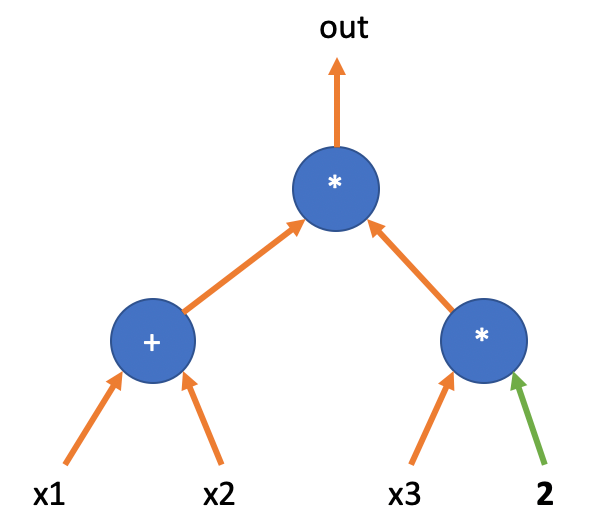
\includegraphics[scale=0.3]{img/img20230414162317.png}


这个电路表示了这样的一个计算:

\[
(x_1 + x_2) \cdot (2\cdot x_3) = out
\]

电路中有4个变量,其中三个变量为输入变量 \((x_1, x_2, x_3)\)
,一个输出变量 \(out\),其中还有一个输入为常数,其值为 \(2\)。

一个电路有两种状态:「空白态」和「运算态」。当输入变量没有具体值的时候,电路处于「空白态」,这时我们只能描述电路引线之间的关系,即电路的结构拓扑。

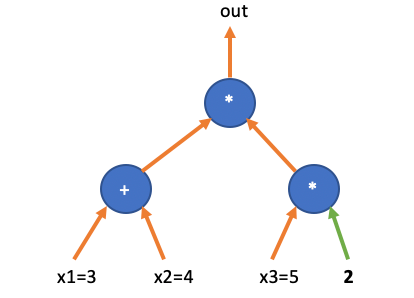
\includegraphics[scale=0.5]{img/img20230414162845.png}

接下来的问题是,我们要先编码电路的「空白态」,即编码各个门的位置,和他们之间引线连接关系。

R1CS
是通过图中的乘法门为中心,用三个「选择子」矩阵来「选择」乘法门的「左输入」、「右输入」、「输出」都分别连接了那些变量。

我们先看看图中最上面的乘法门的左输入,可以用下面的表格来描述:

\[
\begin{array}{|c|c|c|c|c|}
\hline
1 & x_1 & x_2 & x_3 & out \\
\hline
0 & 1 & 1 & 0 & 0 \\
\hline
\end{array}
\]

这个表格只有一行,因此我们可以用一个向量 \(U=(0,1,1,0,0)\)
来代替,表示乘法门的左输入连接了两个变量,\(x1\) 和
\(x_2\)。记住,所有的加法门都会被展开成多个变量的相加(或线性组合)。

再看看其右输入,连接了一个变量 \(x_3\) 和一个常数值,等价于连接了
\(x_3\) 的两倍,那么右输入的选择子矩阵可以记为

\[
\begin{array}{|c|c|c|c|c|}
\hline
1 & x_1 & x_2 & x_3 & out \\
\hline
0 & 0 & 0 & 2 & 0 \\
\hline
\end{array}
\]

这里同样可以用一个行向量 \(V=(0,0,0,2,0)\) 来表示,其中的 \(2\)
即为上图中电路的常数引线。

最后乘法门的输出按照上面的方法可以描述为 \(W=(0,0,0,0,1)\),即输出变量为
\(out\):

\[
\begin{array}{|c|c|c|c|c|}
\hline
1 & x_1 & x_2 & x_3 & out \\
\hline
0 & 0 & 0 & 0 & 1 \\
\hline
\end{array}
\]

有了三个向量 \((U,V,W)\),我们可以通过一个「内积」等式来约束电路的运算:

\[
\big(U\cdot(1,x_1, x_2,x_3,out)\big) \cdot \big(V\cdot(1,x_1, x_2,x_3,out)\big) = \big(W\cdot(1,x_1, x_2,x_3,out)\big)
\]

这个等式化简之后正好可以得到:

\[
(x_1 + x2) \cdot (2\cdot x_3) = out
\]

如果我们把这几个变量换成赋值向量
\((1,x_1,x_2,x_3,out) = (1,3,4,5,70)\),那么电路的运算可以通过「内积」等式来验证:

\[
(U\cdot(1,3,4,5,70))\cdot(U\cdot(1,3,4,5,70))=W\cdot(1,3,4,5,70)
\]

而一个错误的赋值向量,比如 \((1,3,4,\fbox{0},70)\)
,则不满足「内积等式」:

\[
(U\cdot(1,3,4,\fbox{0},70))\cdot(U\cdot(1,3,4,\fbox{0},70))\neq W\cdot(1,3,4,\fbox{0},70)
\]

左边运算结果为 \(0\),右边运算结果为 \(70\)。当然,我们可以验证
\((1,3,4,0,0)\) 也是一组合法(满足电路约束)的赋值。

并不是任何一个电路都存在赋值向量。凡是存在合法的赋值向量的电路,被称为可被满足的电路。判断一个电路是否可被满足,是一个
NP-Complete 问题,也是一个 NP 困难问题。

这里例子中的两个乘法门并不相同,上面的乘法门是左右输入中都含有变量,而下面的乘法门只有一边的输入为变量,另一边为常数。对于后者这类「常数乘法门」,后续我们也把他们看作为特殊的「加法门」,如下图所示,左边电路右下的乘法门等价于右边电路的右下加法门。

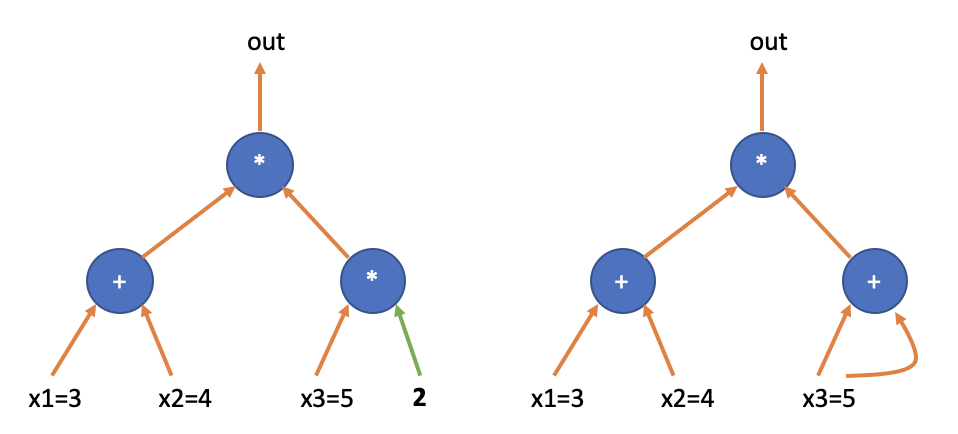
\includegraphics[scale=0.5]{img/img20230423133455.png}

那么如果一个电路含有两个以上的乘法门,我们就不能用 \(U,V,W\)
三个向量之间的内积关系来表示运算,而需要构造「三个矩阵」的运算关系。

\hypertarget{ux591aux4e2aux4e58ux6cd5ux95e8}{%
\subsection{多个乘法门}\label{ux591aux4e2aux4e58ux6cd5ux95e8}}

比如下图所示电路,有两个乘法门,他们的左右输入都涉及到变量。

%\includegraphics{img/img20230414170601.png}

这个电路表示了这样的一个计算:

\[
(x_1 + x2) \cdot (x3 \cdot x4) = out
\]

我们以\textbf{乘法门}为基准,对电路进行编码。第一步将电路中的乘法门依次编号(无所谓编码顺序,只要前后保持一致)。图中的两个乘法门编码为
\texttt{\#1} 与 \texttt{\#2}。

然后我们需要为每一个乘法门的中间值引线也给出变量名:比如四个输入变量被记为
\(x_1, x_2, x_3, x_4\),其中 \(x_5\)
为第二个乘法门的输出,同时作为第一个乘法门的右输入。而 \(out\)
为第一个乘法门的输出。于是我们可以得到一个关于变量名的向量:

\[
(x_1, x_2, x_3, x_4, x_5, out)
\]

该电路的「空白态」可以用下面的三个矩阵来编码:

\[
U, V, W \in \mathbb{F}^{n\times m}
\]

其中 \(n\) 为乘法门的数量,而 \(m\) 大致为引线的数量。每一个矩阵的第
\(i\) 行「选择」了第 \(i\)
个乘法门的输入输出变量。比如我们定义电路的左输入矩阵 \(U\) :

$$
\begin{array}{|c|c|c|c|c|cc}
\hline x_1 & x_2 & x_3 & x_4 & x_5 & \text { out } & \text { i } \\
\hline 1 & 1 & 0 & 0 & 0 & 0 & 1 \\
\hline 0 & 0 & 1 & 0 & 0 & 0 & 2 \\
\hline
\end{array}
$$

其中第一个乘法门的左输入为 \((x_1+x_2)\), 第二个乘法门的左输入为
\(x_3\)。右输入矩阵 \(V\) 定义为:

$$
\begin{array}{|c|c|c|c|c|cc}
\hline x_1 & x_2 & x_3 & x_4 & x_5 & \text { out } & \text { i } \\
\hline 0 & 0 & 0 & 0 & 1 & 0 & 1 \\
\hline 0 & 0 & 0 & 1 & 0 & 0 & 2 \\
\hline
\end{array}
$$

其中1号门的右输入为 \(x_5\),第二个乘法门的右输入为
\(x_4\)。最后定义输出矩阵 \(W\):

$$
\begin{array}{|c|c|c|c|c|cc}
\hline x_1 & x_2 & x_3 & x_4 & x_5 & \text { out } & \text { i } \\
\hline 0 & 0 & 0 & 0 & 0 & 1 & 1 \\
\hline 0 & 0 & 0 & 0 & 1 & 0 & 2 \\
\hline
\end{array}
$$

我们把所有的引线赋值看作为一个向量: \(\vec{a}\) (这里用字母
\(a\),取自 Assignments 首字母)

在上面的例子中,「赋值向量」为

\[
\vec{a} = (x_1, x_2, x_3,x_4,x_5,out)
\]

于是我们可以轻易地检验下面的等式

\[
(U \cdot \vec{a}) \circ (V \cdot \vec{a}) = (W \cdot\vec{a})
\]

其中符号 \(\circ\) 为 Hadamard
Product,表示「按位乘法」。展开上面的按位乘法等式,我们可以得到这个电路的运算过程:

\[
\left[
\begin{array}{c}
x_1 + x_2 \\
x_3 \\
\end{array}
\right]
\circ
\left[
\begin{array}{c}
x_5 \\
x_4 \\
\end{array}
\right]=
\left[
\begin{array}{c}
out \\
x_5 \\
\end{array}
\right]
\]

请注意,通常「赋值向量」中需要一个固定赋值为 \(1\)
的变量,这是为了处理加法门中的常量输入。

\hypertarget{ux4f18ux7f3aux70b9}{%
\subsection{优缺点}\label{ux4f18ux7f3aux70b9}}

由于 R1CS 编码以乘法门为中心,于是电路中的加法门并不会增加 \(U, V, W\)
矩阵的行数,因而对 Prover 的性能影响不大。R1CS
电路的编码清晰简单,利于在其上构造各种 SNARK 方案。

在 2019 年 Plonk
论文中的编码方案同时需要编码加法门与乘法门,看起来因此会增加约束的数量,降低
Proving 性能。但 Plonk
团队随后陆续引入了除乘法与加法外的运算门,比如实现范围检查的门,实现异或运算的门等等。不仅如此,Plonk
支持任何其输入输出满足多项式关系的门,即 Custom Gate,还有适用于实现 RAM
的状态转换门等,随着查表门的提出,Plonk
方案逐步成为许多应用的首选方案,其编码方式也有了一个专门的名词:Plonkish。

\hypertarget{plonkish-ux7b97ux672fux95e8}{%
\section{Plonkish 算术门}\label{plonkish-ux7b97ux672fux95e8}}

回看下例子电路,我们把三个门全都编号,
\(\texttt{1},\texttt{2},\texttt{3}\),同时把加法门的输出值也标记为变量
\(x_6\)。

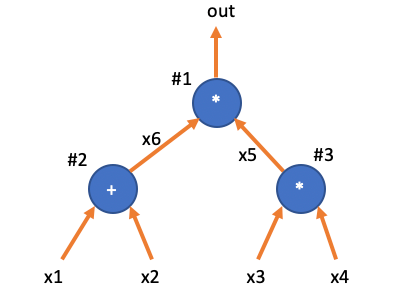
\includegraphics{img/img20230414202348.png}

显然,上面的电路满足三个约束:

\begin{itemize}
\item
  \(x_1 + x_2 =x_6\)
\item
  \(x_3\cdot x_4 = x_5\)
\item
  \(x_6 \cdot x_5 = out\)
\end{itemize}

我们定义一个矩阵 \(W\in\mathbb{F}^{n\times 3}\) 来表示约束( \(n\)
为算术门的数量):

\[
\begin{array}{c|c|c|c|}
\texttt{i} & w_a & w_b & w_c  \\
\hline
\texttt{1} & x_6 & x_5 & out \\
\texttt{2} & x_1 & x_2 & x_6 \\
\texttt{3} & x_3 & x_4 & x_5 \\
\end{array}
\]

为了区分加法和乘法,我们再定一个向量 \(Q\in\mathbb{F}^{n\times5}\)
来表示运算符

$$
\begin{array}{c|c|c|c|cc}
i & q_L & q_R & q_M & q_C & q_O \\
\hline 1 & 0 & 0 & 1 & 0 & 1 \\
2 & 1 & 1 & 0 & 0 & 1 \\
3 & 0 & 0 & 1 & 0 & 1
\end{array}
$$

于是我们可以通过下面的等式来表示三个约束:

\[
q_L \circ w_a + q_R \circ w_b + q_M\circ(w_a\cdot w_b) + q_C -  q_O\circ w_c = 0
\]

如果把上面的等式代入并展开,我们可以得到下面的约束等式:

\[
\left[
\begin{array}{c}
0\\
1 \\
0\\
\end{array}
\right]
\circ
\left[
\begin{array}{c}
x_6 \\
x_1 \\
x_5\\
\end{array}
\right]
+
\left[
\begin{array}{c}
0\\
1 \\
0\\
\end{array}
\right]
\circ
\left[
\begin{array}{c}
x_5 \\
x_2 \\
x_4\\
\end{array}
\right]
+
\left[
\begin{array}{c}
1\\
0 \\
1\\
\end{array}
\right]
\circ
\left[
\begin{array}{c}
x_6\cdot x_5 \\
x_1\cdot x_2 \\
x_3\cdot x_4\\
\end{array}
\right]=\left[
\begin{array}{c}
1\\
1 \\
1\\
\end{array}
\right]
\circ
\left[
\begin{array}{c}
out \\
x_6 \\
x_5\\
\end{array}
\right]
\]

化简后得:

\[
\left[
\begin{array}{c}
0 \\
x_1 \\
0\\
\end{array}
\right]
+
\left[
\begin{array}{c}
0 \\
x_2 \\
0\\
\end{array}
\right]
+
\left[
\begin{array}{c}
x_6\cdot x_5 \\
0 \\
x_3\cdot x_4\\
\end{array}
\right]=\left[
\begin{array}{c}
out \\
x_6 \\
x_5\\
\end{array}
\right]
\]

这正好是三个算术门的计算约束。

总结下,Plonkish 需要一个矩阵 \(Q\)
来描述电路空白态,而所有的赋值则写入了 \(W\) 矩阵。对于 Prover 和
Verifier 的交换协议,\(W\) 是 Prover 的 witness,属于秘密知识,对
Verifier 保密, \(Q\) 矩阵代表了一个实现双方约定共识的电路描述。

不过仅仅有 \(Q\) 矩阵是不足以精确描述上面的例子电路。

\hypertarget{ux590dux5236ux7ea6ux675f}{%
\section{复制约束}\label{ux590dux5236ux7ea6ux675f}}

比较下面两个电路,它们的 \(Q\) 矩阵完全相同,但它们却完全不同。

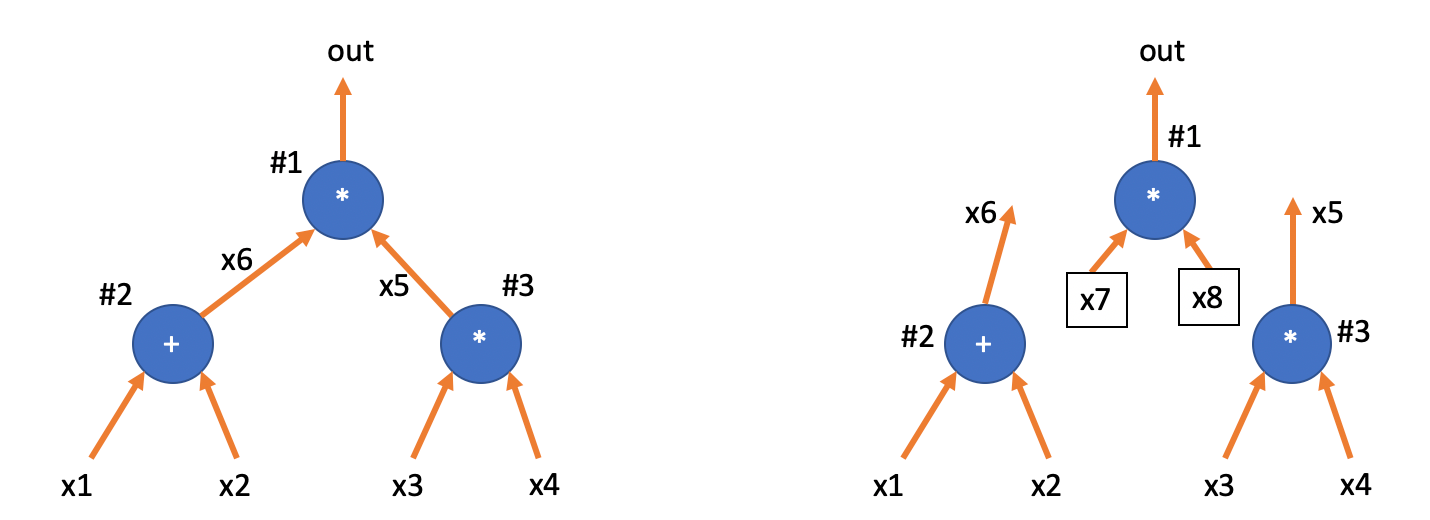
\includegraphics[scale=0.3]{img/img20230414205219.png}

两个电路的区别在于 \(x_5, x_6\) 是否被接入了 \texttt{\#1} 号门。如果让
Prover 直接把电路赋值填入 \(W\) 表格,一个「诚实的」Prover 会在
\(w_{a,1}\) 和 \(w_{c,2}\) 两个位置填上相同的值;而一个「恶意的」Prover
完全可以填上不同的值。如果恶意 Prover 在 \(w_{b,1}\) 和 \(w_{c,3}\)
也填入不同的值,那么实际上 Prover 证明的是上图右边的电路,而非是和
Verifier 共识过的电路(左边)。

$$
\begin{array}{c|c|c|c|}
i & w_a & w_b & w_c \\
\hline 1 & \boxed{x_6} & \underline{x_5} & \text { out } \\
2 & x_1 & x_2 & \boxed{x_6} \\
3 & x_3 & x_4 & \underline{x_5}
\end{array}
$$

我们需要增加新的约束,强制要求右边电路图中 \(x_6=x_7\) 和
\(x_5=x_8\)。这等价于我们要求 Prover
把同一个变量填入表格多个位置时,\textbf{必须填入相等的值}。

这就需要一类新的约束------「拷贝约束」,即 Copy Contraint。Plonk
采用「置换证明」保证 \(W\)
表格中多个位置上的值满足拷贝关系。我们继续用上面这个电路图的案例来说明其基本思路:

设想我们把 \(W\) 表格中的所有位置索引排成一个向量:

\[
\sigma_0=(\boxed{w_{a,1}}, w_{a,2}, w_{a,3}, \underline{w_{b,1}}, w_{b,2}, w_{b,3}, w_{c,1}, \boxed{w_{c,2}}, \underline{w_{c,3}})
\]

然后把应该相等的两个位置互换,比如上图中要求 \(w_{a,1}=w_{c,2}\) 和
\(w_{b,1}=w_{c,3}\) 。于是我们得到了下面的位置向量:

\[
\sigma=(\boxed{w_{c,2}}, w_{a,2}, w_{a,3}, \underline{w_{c,3}}, w_{b,2}, w_{b,3}, w_{c,1}, \boxed{w_{a,1}}, \underline{w_{b,1}})
\]

然后我们要求 Prover 证明:\textbf{\(W\)
表格按照上面的置换之后,仍然等于自身}。置换前后的相等性可以保证 Prover
无法作弊。

再来一个例子,当约束一个向量中有三个(或多个)位置上的值必须相同时,只需要把这三个(或多个)位置的值进行循环移位(左移位或者右移位),然后证明移位后的向量与原向量相等即可。比如:

\[
A = (b_1, b_2, \underline{a_1}, b_3, \underline{a_2}, b_4, \underline{a_3})
\]

如果要证明 \(a_1=a_2=a_3\),那么只需要证明:

\[
A' =  (b_1, b_2, \underline{a_3}, b_3, \underline{a_1}, b_2, \underline{a_2}) \overset{?}{=} A
\]

在经过置换的向量 \(A'\) 中, \(a_1, a_2, a_3\) 依次右移交换,即 \(a_1\)
放到了原来 \(a_2\) 的位置,而 \(a_2\) 放到了 \(a_3\) 的位置, \(a_3\)
则放到了 \(a_1\) 的位置。

如果 \(A'=A\) ,那么 \(A'\) 和 \(A\)
所有对应位置上的值都应该相等,可得: \(a_1=a_4\), \(a_2=a_1\),
\(a_3=a_2\),即
\(a_1=a_2=a_3\)。这个方法可以适用于任意数量的等价关系。(后续证明两个向量相等的方法请见下章)

那么如何描述电路赋值表格中的交换呢?我们只需要记录 \(\sigma\)
向量即可,当然 \(\sigma\) 向量也可以写成表格的形式:

\[
\begin{array}{c|c|c|c|}
i & \sigma_a & \sigma_b & \sigma_c  \\
\hline
1 & \boxed{w_{c,2}} & \underline{w_{c,3}}& w_{c,1} \\
2 & w_{a,2} & w_{b,2} & \boxed{w_{a,1}} \\
3 & w_{a,3} & w_{b,3} & \underline{w_{b,1}} \\
\end{array}
\]

加上 \(\sigma\) ,空白电路可以描述为 \((Q,\sigma)\) ,电路的赋值为 \(W\)

\[
\mathsf{Plonkish}_0 \triangleq (Q, \sigma; W)
\]

\hypertarget{ux518dux6bd4ux8f83}{%
\section{再比较}\label{ux518dux6bd4ux8f83}}

R1CS 的 \((U,V,W)\)
表格的宽度与引线的数量有关,行数跟乘法门数量有关。这个构造相当于把算术电路看成是仅有乘法门构成,但每个门有多个输入引脚(最多为所有引线的数量)。而
Plonkish 则是同等对待加法门与乘法门,并且因为输入引脚只有两个, 所以
\(W\)
表格的宽度固定,仅有三列(如果要支持高级的计算门,表格可以扩展到更多列)。这一特性是
Plonk 可以利用 Permutation Argument 实现拷贝约束的前提。

\begin{quote}
\ldots, and thus our linear contraints are just wiring constraints that
can be reduced to a permutation check.
\end{quote}

按照 Plonk
论文的统计,一般情况下,算术电路中加法门的数量是乘法门的两倍。如果这样看来,
\(W\) 表格的长度会三倍于 R1CS
的矩阵。但这个让步会带来更多的算术化灵活度。

\hypertarget{ux7535ux8defux9a8cux8bc1ux534fux8baeux6846ux67b6}{%
\section{电路验证协议框架}\label{ux7535ux8defux9a8cux8bc1ux534fux8baeux6846ux67b6}}

有了电路空白结构的描述和赋值,我们可以大致描述下 Plonk 的协议框架。

首先 Prover 和 Verifier 会对一个共同的电路进行共识, \((Q,\sigma)\) 。
假设电路的公开输出为 \(out=99\),而 \((x_1,x_2,x_3,x_4)\) 为秘密输入。

Prover 填写 \(W\) 矩阵(Verifier 不可见):

\[
\begin{array}{c|c|c|c|}
i & w_a & w_b & w_c  \\
\hline
1 & \boxed{x_6} & \underline{x_5} & [out] \\
2 & x_1 & x_2 & \boxed{x_6} \\
3 & x_3 & x_4 & \underline{x_5} \\
4 & 0 & 0 & [out] \\
\end{array}
\]

其中增加的第四行是为了增加一个额外的算术约束: \(out=99\) ,把 \(out\)
值显示地表示在 \(Q\) 矩阵中。

相应的那么 Prover 和 Verifier 共识的 \(Q\) 矩阵为

\[
\begin{tabular}{c|c|c|c|cc}
    $i$ & $q_L$ & $q_R$ & $q_M$ & $q_C$ & $q_O$ \\
    \hline 1 & 0 & 0 & 1 & 0 & 1 \\
    2 & 1 & 1 & 0 & 0 & 1 \\
    3 & 0 & 0 & 1 & 0 & 1 \\
    4 & 0 & 0 & 0 & 99 & 1
\end{tabular}
\]

其中第四行约束,保证 \(out=99\),可以把
\((q_L=0, q_R=0,q_M=0,q_C=99,q_O=1)\) 代入下面的算术约束,可得
\(99-w_c = 0\) ,即 \(w_{c,4}=99\) 。

\[
q_L \circ w_a + q_R \circ w_b + q_M\circ(w_a\cdot w_b) + q_C -  q_O\circ w_c = 0
\]

为了保证第一行的 \(w_c\) 也必须为 \(99\),这就需要在 \(\sigma\)
矩阵中添加额外的一条拷贝约束:让 \(out\) 变量的位置 \((w_{c,1})\) 与
第四行的输出 \(w_{c,4}\) 交换对调:

\[
\begin{array}{c|c|c|c|}
i & \sigma_a & \sigma_b & \sigma_c  \\
\hline
1 & \boxed{w_{c,2}} & \underline{w_{c,3}} & [w_{c,4}] \\
2 & w_{a,2} & w_{b,2} & \boxed{w_{a,1}} \\
3 & w_{a,3} & w_{b,3} & \underline{w_{b,1}} \\
4 & w_{a,4} & w_{b,4} & [w_{c,1}]\\
\end{array}
\]

如果 Prover 是诚实的,那么对于
\(i\in(1,2,3,4)\),下面的算术约束等式成立:

\[
q_{L,i} \circ w_{a,i} + q_{R,i} \circ w_{b,i} + q_{M,i}\circ(w_{a,i}\cdot w_{b,i}) + q_{C,i} -  q_{O,i}\circ w_{c,i} = 0
\]

验证协议的大概思路如下:

协议开始:Prover 如实填写 \(W\) 表格,然后把 \(W\)
表格的每一列进行编码,并进行多项式编码,并把编码后的结果发送给 Verifier

协议验证阶段:Verifier 与 Prover
通过进一步的交互,验证下面的等式是否成立:

\[
q_{L}(X) \cdot w_{a}(X) + q_{R}(X) \cdot w_{b}(X) + q_{M}(X)\cdot(w_{a}(X)\cdot w_{b}(X)) + q_{C}(X) -  q_{O}(X)\cdot w_{c}(X) \overset{?}{=} 0
\]

当然这个验证还不够,还要验证 \((\sigma_a(X),\sigma_b(X),\sigma_c(X))\)
与 \((w_a(X),w_b(X),w_c(X))\) 之间的关系。还有,Verifier
如何通过多项式来验证电路的运算,请看后续章节。

% \hypertarget{ux53c2ux8003ux6587ux732e}{%
% \subsection{参考文献}\label{ux53c2ux8003ux6587ux732e}}

% \begin{itemize}
% \tightlist
% \item
%   {[}BG12{]} Bayer, Stephanie, and Jens Groth. ``Efficient
%   zero-knowledge argument for correctness of a shuffle.'' \emph{Annual
%   International Conference on the Theory and Applications of
%   Cryptographic Techniques}. Springer, Berlin, Heidelberg, 2012.
% \item
%   {[}GWC19{]} Ariel Gabizon, Zachary J. Williamson, and Oana Ciobotaru.
%   ``Plonk: Permutations over lagrange-bases for oecumenical
%   noninteractive arguments of knowledge.'' \emph{Cryptology ePrint
%   Archive} (2019).
% \end{itemize}




\hypertarget{ux7406ux89e3-plonkux4e8cux591aux9879ux5f0fux7f16ux7801}{%
\chapter{多项式编码}\label{ux7406ux89e3-plonkux4e8cux591aux9879ux5f0fux7f16ux7801}}

在上篇文章里,我们可以把电路的计算的「合法性检查」转换成一组加法/乘法约束。假如总共有
N 个约束,那么Prover
可以通过多项式编码的方式把多个约束压缩成一个约束,让 Verifier 轻松检查。

\hypertarget{ux591aux9879ux5f0fux7684ux6982ux7387ux68c0ux67e5}{%
\section{多项式的概率检查}\label{ux591aux9879ux5f0fux7684ux6982ux7387ux68c0ux67e5}}

把多个约束验证合并的神奇能力来自于「多项式随机挑战」。如果有两个多项式
\(f(X)\) 和 \(g(X)\) 同为两个次数不超过 \(d\) 的多项式。那么 Verifier
只需要给出一个随机挑战值 \(\zeta\in \mathbb{F}\),计算 \(f(\zeta)\)
是否等于 \(g(\zeta)\) 即可大概率得知 \(f(X)=g(X)\),其中出错的概率
\(\leq\frac{d}{|\mathbb{F}|}\)。只要保证 \(\mathbb{F}\)
足够大,那么检查出错的概率就可以忽略不计。

这个原理被称为 Schwartz-Zippel 定理。 \footnote{Schwartz–Zippel lemma. \url{https://en.wikipedia.org/wiki/SchwartzZippel_lemma}}

假如要验证两个向量 \(\vec{a} + \vec{b}\) 是否等于
\(\vec{c}\),为了可以一步挑战验证,我们要先把三个向量编码成多项式。

一种最直接的方案是把向量当作多项式的「系数」进行编码

\[
\begin{split}
a(X) &= a_0 + a_1X+a_2X^2 + \cdots + a_{n-1}X^{n-1}\\
b(X) &= b_0 + b_1X+b_2X^2 + \cdots + b_{n-1}X^{n-1}\\
c(X) &= c_0 + c_1X+c_2X^2 + \cdots + c_{n-1}X^{n-1}
\end{split}
\]

显然,如果 \(a_i+ b_i = c_i\),那么
\(a(X)+b(X)=c(X)\)。然后我们可以通过挑战一个随机数 \(\zeta\)
来检验三个多项式在 \(X=\zeta\) 处的取值,验证:

\[
a(\zeta)+b(\zeta)\overset{?}{=}c(\zeta) 
\]

如果上式成立,那么 \(\vec{a} + \vec{b}=\vec{c}\) 。

\hypertarget{lagrange-ux63d2ux503c-ux4e0e-evaluation-form}{%
\section{Lagrange 插值 与 Evaluation
Form}\label{lagrange-ux63d2ux503c-ux4e0e-evaluation-form}}

假如我们要验证
\(\vec{a}\circ\vec{b}\overset{?}{=}\vec{c}\),用系数编码的方式就不容易处理了,因为
\(a(X)\cdot b(X)\) 会产生很多的交叉项。并且 \(a_i\cdot b_i\) 和 \(c_i\)
的项并不对应到 \(X^i\) 的系数,比如 \(a_1\cdot b_1\) 的系数出现在
\(X^2\) 上,但同时 \(X^2\) 项的系数组成还有 \(a_0\cdot b_2\) 和
\(a_2\cdot b_0\)。而 \(c_1\) 是 \(X^1\) 的系数。

我们需要另一种多项式编码方案,利用 Lagrange Basis。如果我们要构造多项式
\(a(X)\),使得它在定义域 \(H=(w_0, w_1, \ldots w_{N-1})\) 上的取值为
\(\vec{a}\),即

\[
\begin{split}
a(w_0) &= a_0 \\
a(w_1) &= a_1 \\
&\vdots \\
a(w_{N-1}) &= a_{N-1} \\
\end{split}
\]

插值需要用到一组插值多项式: \(\{L_i(X)\}_{i\in[0,N-1]}\),其中
\(L_i(w_i)=1\),并且 \(L_i(w_j)=0 (j\neq i)\)。然后 \(\vec{a}\)
可以按如下方式编码:

\[
a(X)=a_0\cdot L_0(X) + a_1\cdot L_1(X)+ a_2\cdot L_2(X) + \cdots + a_{N-1}\cdot L_{N-1}(X)
\]

可以简单心算一下,当 \(X=w_0\)
时,等式右边除了第一项之外,其他项都等于零,于是 \(a(w_0)=a_0\)。看起来
\(L_i(X)\) 像是一个选择器,这组多项式又被称为 Lagrange Polynomials。

我们用同样的方法来编码 \(b(X)\) 和 \(c(X)\):

\[
\begin{split}
b(X)=b_0\cdot L_0(X) + b_1\cdot L_1(X)+ b_2\cdot L_2(X) + \cdots + b_{N-1}\cdot L_{N-1}(X) \\
c(X)=c_0\cdot L_0(X) + c_1\cdot L_1(X)+ c_2\cdot L_2(X) + \cdots + c_{N-1}\cdot L_{N-1}(X) \\
\end{split}
\]

如果 \(a_i\cdot b_i = c_i\) 成立,那么
\(a(w_i)\cdot b(w_i) = c(w_i)\)。如果 \(\vec{a}\circ\vec{b}{=}\vec{c}\)
,那么

\[
a(X)\cdot b(X) = c(X),\quad \forall X\in H
\]

我们现在已经把两个向量的按位乘积问题转换到了三个多项式之间的关系,接下来的问题是如何进行随机挑战验证。

我们发现:如果直接让 Verifier 发送随机数 \(\zeta\) 挑战上面的等式,那么
\(\zeta\) 只能属于 \(H\)。如果只存在一个 \(j\) 使得
\(a_j\cdot b_j\neq c_j\),那么 Verifier
的一次挑战能发现这个错误的概率只有 \(\frac{1}{|n|}\),这样 Verifier
需要挑战多次才能缩小检测出错的概率。不过这样不满足我们的要求,我们希望只通过一次挑战来检测出
Prover 的作弊行为。

我们可以把上面的等式的 \(X\) 取值范围去除,换成下面的等式:

\[
a(X)\cdot b(X) - c(X) = q(X)\cdot z_H(X), \quad\forall X\in \mathbb{F}
\]

这个等式在整个 \(\mathbb{F}\) 定义域上都成立。这是为何?

首先我们看等式左边的多项式: \(a(X)\cdot b(X)-c(X)\),不妨定义为
\(f(X)\)。我们可以看到 \(f(X)\) 在 \(X\in H\) 上等于零,那么意味着 \(H\)
恰好是 \(f(X)\) 的「根集合」。于是 \(f(X)\)
可以按照下面的方式进行因式分解:

\[
f(X)=(X-w_0)(X-w_1)(X-w_2)\cdots(X-w_{N-1})\cdot q(X)
\]

换个说法, \(f(X)\) 可以被多项式
\(z_H(X)=(X-w_0)(X-w_1)(X-w_2)\cdots(X-w_{n-1})\)
整除,并得到一个商多项式 \(q(X)\)。零多项式 \(z_H(X)\) 又被称为
Vanishing Polynomial。

如果我们让 Prover 计算出这个 \(q(X)\),并且发送给 Verifier,又因为 \(H\)
是已知的系统参数,Verifier 可以自行计算 \(z_H(X)\),那么 Verifier
只需要一次随机检测即可判断 \(a(X)\cdot b(X)-c(X)\) 是否在 \(H\) 处等零。

\[
a(\zeta)\cdot b(\zeta)-c(\zeta) \overset{?}{=} q(\zeta)\cdot z_H(\zeta)
\]

进一步,如果我们使用多项式承诺(Polynomial Commitment),Verifier 可以让
Prover 来帮忙计算这些多项式在 \(X=\zeta\)
处的取值,发送并证明这些值的正确性,这样能最大限度地减少 Verifier
的工作量。

但是, Verifier 计算 \(z_H(\zeta)\) 需要 \(O(n)\) 的计算量。

那能否让 Verifier 继续减少工作量?答案是可以的,只要我们选择特殊的
\(H\subset \mathbb{F}\) 。

\hypertarget{ux5355ux4f4dux6839-roots-of-unity}{%
\section{单位根 Roots of
Unity}\label{ux5355ux4f4dux6839-roots-of-unity}}

如果我们选择单位根作为 \(H\),那么 \(z_H(\zeta)\) 的计算量会降为
\(O(\log{n})\)。

对于任何有限域 \(\mathbb{F}_p=(0,1,\ldots,p-1)\),其中阶数 \(p\)
为素数。那么去除零之后剩下的元素构成了乘法群
\(\mathbb{F}_p^\ast=(1,\ldots,p-1)\),阶数为 \(p-1\)。由于 \(p-1\)
一定为偶数,那么 \(p-1\) 的乘法因子中一定包含若干个 \(2\),假设记为
\(\lambda\) 个 \(2\)。那么 \(\mathbb{F}_p^\ast\) 一定包含一个阶数为
\(2^\lambda\) 的乘法子群。不妨设
\(n=2^{k}, k\leq\lambda\),那么一定存在一个阶数为 \(n\) 的乘法子群,记为
\(H\)。 该乘法子群必然含有一个生成元,记为 \(\omega\),并且
\(\omega^N=1\)。这相当于把 \(1\) 开 \(N\)
次方根,因此被称为单位根。不过单位根不只有一个 \(\omega\),我们会发现
\(\omega^2,\omega^3,\ldots,\omega^{N-1}\) 都满足单位根的特性,即
\((\omega^k)^N=1, k\in(2,3,\ldots,N-1)\)。那么所有这些由 \(\omega\)
产生的单位根就组成了乘法子群 \(H\):

\[
H=(1,\omega,\omega^2,\omega^3,\ldots,\omega^{N-1})
\]

这些元素满足一定的对称性:比如 \(\omega^{\frac{N}{2}}=-1\) ,
\(\omega=-\omega^{\frac{N}{2}+1}\),
\(\omega^i=-\omega^{\frac{N}{2}+i}\)。又比如把所有的单位根求和,我们会得到零:

\[
\sum_{i=0}^{N-1}\omega^i=0
\]

举一个简单的例子,我们可以在 \(\mathbb{F}_{13}\) 中找到一个阶数为 \(4\)
的 \(H\)。

\[
\mathbb{F}_{13}=(0,1,2,3,4,5,6,7,8,9,10,11,12)
\]

其中乘法群的生成元为 \(g=2\)。由于 \(13-1=3*2*2\),所以存在一个阶数为
\(4\) 的乘法子群,其生成元为 \(\omega=5\):

\[
H=(\omega^0=1,\omega^1=5,\omega^2=12,\omega^3=8)
\]

而 \(\omega^4=1=\omega^0\)。

在实际应用中,我们会选择一个较大的有限域,它能有一个较大的 Powers-of-2
乘法子群。比如椭圆曲线 \texttt{BN254} 的 Scalar Field,含有一个阶数为
\(2^{28}\) 的乘法子群,\texttt{BLS-12-381} 的Scalar Field 含有一个阶数为
\(2^{32}\) 的乘法子群。

在乘法子群 \(H\) 上,具有下面的性质:

\[
z_H(X)=\prod_{i=0}^{N-1}(X-\omega^i)=X^N-1
\]

我们可以进行简单的推导,假设 \(N = 4\),由于 \(\omega^i\)
的对称性,这个计算过程可以不断化简:

\[
\begin{split}
&(X-\omega^0)(X-\omega^1)(X-\omega^2)(X-\omega^3) \\
=& (X-1)(X-\omega)(X+1)(X-\omega^{3})  \\
=& (X^2-1)(X-\omega)(X+\omega) \\
=& (X^2-1)(X^2-\omega^2) \\
=& (X^2-1)(X^2+1) \\
=& (X^4-1) \\
\end{split}
\]

\hypertarget{lagrange-basis}{%
\section{Lagrange Basis}\label{lagrange-basis}}

对于 Lagrange 多项式, \(L_i(w_i)=1\),并且
\(L_i(w_j)=0, (j\neq i)\)。接下来,我们给出 \(L_i(X)\) 的构造。

为了构造 \(L_i(X)\),先构造不等于零的多项式部分。由于
\(L_i(\omega_j)=1, j = i\),因此他一定包含
\(\prod_{j,j\neq i}(X-\omega_j)\) 这个多项式因子。但该因子显然在
\(X=\omega_i\) 处可能不等于 \(1\),即可能
\(\prod_{j, j\neq i}(\omega_i-\omega_j)\neq 1\)。然后,我们只要让该因子除以这个可能不等于
\(1\) 的值即可,于是 \(L_i(X)\) 定义如下:

\[
L_i(X) = \frac{\prod_{j\in H\backslash\{i\}}(X-\omega_j)}{\prod_{j\in H\backslash\{i\}}(\omega_i-\omega_j)} = \prod_{j\in H\backslash\{i\}}^{} \frac{X-\omega_j}{\omega_i-\omega_j}
\]

不难发现, \(L_i(X)\) 在 \(X=\omega_i\) 处等于 \(1\),其它位置
\(X=\omega_j, j\neq i\) 处等于 \(0\)。

对于任意次数小于 \(N\) 的多项式 \(f(X)\),那么它都可以唯一地表示为:

\[
f(X)=a_0\cdot L_0(X)+a_1\cdot L_1(X)+a_2\cdot L_2(X)+ \cdots + a_{N-1}\cdot L_{N-1}(X)
\]

我们可以用多项式在 \(H\) 上的值 \((a_0,a_1,a_2,\ldots,a_{N-1})\) 来表示
\(f(X)\)。这被称为 多项式的求值形式(Evaluation
Form),区别于系数形式(Coefficient Form)。

两种形式可以在 \(H\) 上可以通过 (Inverse) Fast Fourier Transform
算法来回转换,计算复杂度为 \(O(N\log{N})\)。

\hypertarget{ux591aux9879ux5f0fux7684ux7ea6ux675f}{%
\section{多项式的约束}\label{ux591aux9879ux5f0fux7684ux7ea6ux675f}}

利用 Lagrange Basis 我们可以方便地对各种向量计算进行约束。

比如我们想约束 \(\vec{a}=(h,a_1,a_2,\ldots,a_{N-1})\) 向量的第一个元素为
\(h\)。那么我们可以这个向量进行编码,得到 \(a(X)\),并且进行如下约束:

\[
L_0(X)(a(X)-h) = 0, \quad \forall X\in H
\]

Verifier 可以挑战验证下面的多项式等式:

\[
L_0(X)(a(X)-h) = q(X)\cdot z_H(X)
\]

再比如,我们想约束 \(\vec{a}=(h_1,a_1,a_2,\ldots,a_{N-2},h_2)\)
向量的第一个元素为 \(h_1\),最后一个元素为 \(h_2\),其它元素任意。那么
\(a(X)\) 应该满足下面两个约束。

\[
\begin{split}
L_0(X)\cdot (a(X)-h_1) &= 0, \quad \forall X\in H\\
L_{N-1}(X)\cdot(a(X)-h_2) &= 0, \quad \forall X\in H
\end{split}
\]

那么通过 Verifier 给一个随机挑战数(
\(\alpha\)),上面两个约束可以合并为一个多项式约束:

\[
L_0(X)\cdot (a(X)-h_1) + \alpha\cdot L_{n-1}(X)\cdot(a(X)-h_2) = 0, \quad \forall X\in H
\]

接下来,Verifier 只要挑战下面的多项式等式即可:

\[
L_0(X)\cdot (a(X)-h_1) + \alpha\cdot L_{n-1}(X)\cdot(a(X)-h_2) = q(X)\cdot z_H(X)
\]

如果想验证 \(\vec{a}\) 和 \(\vec{b}\)
两个等长向量除第一个元素之外,其它元素都相等,那要如何约束呢?假设
\(a(X)\) 和 \(b(X)\) 为两个向量的多项式编码,那么它们应该满足:

\[
(X-\omega^0)(a(X)-b(X))=0
\]

当 \(X=\omega^0\) 时,左边多项式的第一个因子等于零,而
\(X\in H\backslash\\{\omega^0\\}\)
时,则左边第二因子等于零,即表达了除第一项可以不等之外,其它点取值都必须相等。

可以看出,采用 Lagrange
多项式,我们可以灵活地约束多个向量之间的关系,并且可以把多个约束合并在一起,让
Verifier 仅通过很少的随机挑战就可验证多个向量约束。

\hypertarget{coset}{%
\section{Coset}\label{coset}}

在素数有限域的乘法群中,对于每一个乘法子群
\(H\),都有多个等长的陪集(Coset),这些 Coset 具有和 \(H\)
类似的性质,在 Plonk 中也会用到 Coset 的概念,这里只做部分性质的介绍。

还拿 \(\mathbb{F}_{13}\) 为例,我们取
\(H=(1,5,12,8)\),并且乘法群的生成元 \(g=2\)。于是我们可以得到下面两个
Coset:

$$
\begin{aligned}
& H_1=g \cdot H=\left(g, g \omega, g \omega^2, g \omega^3\right) \quad=(2,10,11,3) \\
& H_2=g^2 \cdot H=\left(g^2, g^2 \omega, g^2 \omega^2, g^2 \omega^3\right)=(4,7,9,6)
\end{aligned}
$$

可以看到
\(\mathbb{F}^*_{13}=H\cup H_1 \cup H_2\),并且它们交集为空,没有任何重叠。并且它们的
Vanishing Polynomial 也可以快速计算:

\[
z_{H_1}(X)=X^N-g^N, \quad z_{H_2}(X)=X^N-g^{2N}
\]

% \hypertarget{references}{%
% \subsection{References}\label{references}}

% \begin{itemize}
% \tightlist
% \item
%   Schwartz--Zippel lemma.
%   https://en.wikipedia.org/wiki/Schwartz\%E2\%80\%93Zippel\_lemma
% \end{itemize}



\hypertarget{ux7406ux89e3-plonkux4e09ux7f6eux6362ux8bc1ux660e}{%
\chapter{置换证明}\label{ux7406ux89e3-plonkux4e09ux7f6eux6362ux8bc1ux660e}} 

Plonkish 电路编码用两个矩阵 \((Q,\sigma)\) 描述电路的空白结构,其中
\(Q\) 为运算开关, \(\sigma\) 为置换关系,用来约束 \(W\)
矩阵中的某些位置必须被填入相等的值。本文重点讲解置换证明(Permutation
Argument)的原理。 \footnote{[WIP] Copy constraint for arbitrary number of wires. \url{https://hackmd.io/CfFCbA0TTJ6X08vHg0-9_g}} 
\footnote{Alin Tomescu. Feist-Khovratovich technique for computing KZG proofs fast. \url{https://alinush.github.io/2021/06/17/Feist-Khovratovich-technique-for-computing-KZG-proofs-fast.html}}
\footnote{Ariel Gabizon. Multiset checks in PLONK and Plookup. \url{https://hackmd.io/@arielg/ByFgSDA7D}}

\hypertarget{ux56deux987eux62f7ux8d1dux5173ux7cfb}{%
\section{回顾拷贝关系}\label{ux56deux987eux62f7ux8d1dux5173ux7cfb}}

回顾一下 Plonkish 的 \(W\) 表格,总共有三列,行数按照 \(2^2\) 对齐。

\[
\begin{array}{c|c|c|c|}
i & w_{a,i} & w_{b,i} & w_{c,i}  \\
\hline
1 & {\color{red}x_6} & {\color{blue}x_5} & {\color{green}out} \\
2 & x_1 & x_2 & {\color{red}x_6} \\
3 & x_3 & x_4 & {\color{blue}x_5} \\
4 & 0 & 0 & {\color{green}out} \\
\end{array}
\]

我们想约束 Prover 在填写 \(W\) 表时,满足下面的拷贝关系:
\(w_{a,1}=w_{c,2}\) \(w_{b,1}=w_{c,3}\) 与
\(w_{c,1}=w_{c,4}\),换句话说, \(w_{a,1}\) 位置上的值需要被拷贝到
\(w_{c,2}\) 处,而 \(w_{b,1}\) 位置上的值需要被拷贝到 \(w_{c,3}\) 处,
\(w_{c,1}\) 位置上的值被拷贝到 \(w_{c,4}\) 处。

问题的挑战性在于,Verifier 要仅通过一次随机挑战就能完成 \(W\)
表格中多个拷贝关系的证明,并且在看不到 \(W\) 表格的情况下。

Plonk 的「拷贝约束」是通过「置换证明」(Permutation
Argument)来实现,即把表格中需要约束相等的那些值进行循环换位,然后证明换位后的表格和原来的表格完全相等。

简化一下问题:如何证明两个等长向量 \(\vec{a}\) 和 \(\vec{a}'\)
满足一个已知的置换 \(\sigma\),并且 \(\vec{a}=\vec{a}'\)

\[
a_i=a'_{\sigma(i)}
\]

举一个例子,假设 \(\vec{a}=(a_0,a_1,a_2,a_3)\),
\(\vec{a}'=(a_1,a_2,a_3,a_0)\),即他们满足一个「左移循环换位」的置换关系,那么
\(\sigma=\\{0\to 1; 1\to 2; 2\to 3; 3\to0\\}\)。如何能证明
\(\vec{a}=\vec{a}'\) ,那么两个向量对应位置的值都应该相等,

\[
\begin{array}{c{|}c|c|c|c|c}
\vec{a} & a_0 & a_1 & a_2 & a_3 \\
\hline
\vec{a}' & a_1 & a_2 & a_3 & a_0 \\
\end{array}
\]

那么 \(a_0=a_1\), \(a_1=a_2\), \(a_2=a_3\),
\(a_3=a_0\),于是可以得出结论: \(a_0=a_1=a_2=a_3\),即 \(\vec{a}\)
中的全部元素都相等。

对于 \(W\) ,我们只需要针对那些需要相等的位置进行循环换位,然后让 Prover
证明 \(W\) 和经过循环换位后的 \(W'\)
表格相等,那么可实现拷贝约束。证明两个表格相等,这个可以通过多项式编码,然后进行概率检验的方式完成。剩下的工作就是如何让
Prover 证明 \(W'\) 确实是(诚实地)按照事先约定的方式进行循环移位。

那么接下来就是理解如何让 Prover 证明两个向量之间满足某一个「置换关系」。
置换证明(Permutation Argument)是 Plonk
协议中的核心部分,为了解释它的工作原理,我们先从一个基础协议开始------连乘证明(Grand
Product Argument)。

\hypertarget{ux51b7ux542fux52a8grand-product}{%
\section{冷启动:Grand
Product}\label{ux51b7ux542fux52a8grand-product}}

假设我们要证明下面的「连乘关系」 :

\[
p = q_0\cdot q_1 \cdot q_2 \cdot \cdots \cdot q_{n-2}
\]

我们在上一篇文章介绍了如何证明一组「单乘法」,通过多项式编码,把多个单乘法压缩成单次乘法的验证。

这里对付连乘的基本思路是:让 Prover
利用一组单乘的证明来实现多个数的连乘证明,然后再通过多项式的编码,交给
Verifier 进行概率检查。

强调下:思路中的关键点是如何把一个连乘计算转换成多次的单乘计算。

我们需要通过引入一个「辅助向量」,把「连乘」的计算看成是一步步的单乘计算,然后辅助向量表示每次单乘之后的「中间值」:

\[
\begin{array}{c|c|l}
q_i & r_i & \ \ q_i\cdot r_i \\
\hline
q_0 & r_0=1  & r_1=q_0\\
q_1 & r_1 & r_2=q_0\cdot q_1\\
q_2 & r_2 & r_3=q_0\cdot q_1\cdot q_2\\
\vdots & \vdots & \vdots\\
q_{n-2} & r_{n-2} & r_{n-1} = p\\
\end{array}
\]

上面表格表述了连乘过程的计算轨迹(Trace),每一行代表一次单乘,顺序从上往下计算,最后一行计算出最终的结果。

表格的最左列为要进行连乘的向量 \({q_i}\),中间列 \({r_i}\)
为引入的辅助变量,记录每次「单乘之前」的中间值,最右列表示每次「单乘之后」的中间值。

不难发现,「中间列」向量 \(\vec{r}\)
向上挪一行与「最右列」几乎一致,除了最后一个元素。该向量的第一个元素用了常数
\(1\) 作为计算初始值,「最右列」最后一个向量元素为计算结果。

向量 \(\vec{r}\) 是一个
Accumulator,即记录连乘计算过程中的每一个中间结果:

\[
r_k = \prod_{i=0}^{k-1}q_i
\]

那么显然我们可以得到下面的递归式:

\[
r_0 = 1, \qquad r_{k+1}=q_{k}\cdot r_{k}
\]

于是,表格的三列编码后的多项式也将满足下面三个约束。第一个是初始值为
\(1\):

\[
L_0(X)\cdot(r(X)-1)=0, \qquad \forall X\in H 
\]

第二个约束为递归的乘法关系:

\[
q(X)\cdot r(X) = r(\omega\cdot X), \qquad \forall X\in H\backslash{\omega^{-1}}
\]

第三个约束最后结果 \(r_{n-1}=p\):

\[
L_{n-1}(X)\cdot(r(X)-p)=0, \qquad \forall X\in H
\]

我们可以用一个小技巧来简化上面的三个约束。我们把计算连乘的表格添加一行,令
\(q_{n-1}=1/p\)(注意: \(p\) 为 \(\vec{q}\) 向量的连乘积)

\[
\begin{array}{c|c|c}
q_i & r_i & q_i\cdot r_i \\
\hline
q_0 & 1  & r_0\\
q_1 & r_0 & r_1\\
q_2 & r_1 & r_2\\
\vdots & \vdots & \vdots\\
q_{n-2} & r_{n-2} & r_{n-1}\\
q_{n-1}=\frac{1}{p} & r_{n-1} & 1 \\
\end{array}
\]

这样一来, \(r_n=r_0=1\) 。最右列恰好是 \(\vec{r}\)
的循环移位。并且上面表格的每一行都满足「乘法关系」!于是,我们可以用下面的多项式约束来表示递归的连乘:

\[
q(X)\cdot r(X)=r(\omega\cdot X), \qquad \forall X\in H
\]

接下来,Verifier 可以挑战下面的多项式等式:

\[
L_0(X)\cdot(r(X)-1)+\alpha\cdot(q(X)\cdot r(X)-r(\omega\cdot X))=h(X)\cdot z_H(X)
\]

其中 \(\alpha\) 是用来聚合多个多项式约束的随机挑战数。其中 \(h(X)\)
为商多项式, \(z_H(X)=(X-1)(X-\omega)\cdots(X-\omega^{n-1})\)。

接下来,通过 Schwartz-Zippel 定理,Verifier 可以给出挑战数 \(\zeta\)
来验证上述多项式等式是否成立。

到此为止,如果我们已经理解了如何证明一个向量元素的连乘,那么接下来的问题是如何利用「连乘证明」来实现「Multiset
等价证明」(Multiset Equality Argument)。

\hypertarget{ux4ece-grand-product-ux5230-multiset-ux7b49ux4ef7}{%
\section{从 Grand Product 到 Multiset
等价}\label{ux4ece-grand-product-ux5230-multiset-ux7b49ux4ef7}}

假设有两个向量,其中一个向量是另一个向量的乱序重排,那么如何证明它们在集合意义(注意:集合无序)上的等价呢?最直接的做法是依次枚举其中一个向量中的每个元素,并证明该元素属于另一个向量。但这个方法有个限制,就是无法处理向量会中出现两个相同元素的情况,也即不支持「多重集合」(Multiset)的判等。例如
\({1,1,2}\) 就属于一个多重集合(Multiset),那么它显然不等于
\({1, 2, 2}\),也不等于 \({2,1}\)。

另一个直接的想法是将两个向量中的所有元素都连乘起来,然后判断两个向量的连乘值是否相等。但这个方法同样有一个严重的限制,就是向量元素必须都为素数,比如
\(3\cdot6=9\cdot2\) ,但 \({3,6}\neq{9,2}\)。

修改下这个方法,我们假设向量 \({q_i}\) 为一个多项式 \(q(X)\)
的根集合,即对向量中的任何一个元素 \(q_i\),都满足
\(q(r_i)=0\)。这个多项式可以定义为:

\[
q(X) = (X-q_0)(X-q_1)(X-q_2)\cdots (X-q_{n-1})
\]

如果存在另一个多项式 \(p(X)\) 等于
\(q(X)\),那么它们一定具有相同的根集合 \({q_i}\)。比如

\[
\prod_{i}(X - q_i) = q(X) = p(X) = \prod_{i}(X - p_i)
\]

那么

\[
\\{q_i\\}=_{multiset}\\{p_i\\}
\]

我们可以利用 Schwartz-Zippel 定理来进一步地检验:向 Verifier
索要一个随机数 \(\gamma\),那么 Prover 就可以通过下面的等式证明两个向量
\({p_i}\) 与 \({q_i}\) 在多重集合意义上等价:

\[
\prod_{{i\in[n]}}(\gamma-p_i)=\prod_{i\in[n]}(\gamma-q_i)
\]

还没结束,我们需要用上一节的连乘证明方案来继续完成验证,即通过构造辅助向量(作为一个累积器),把连乘转换成多个单乘来完成证明。需要注意的是,这里的两个连乘可以合并为一个连乘,即上面的连乘相等可以转换为

\[
\prod_{{i\in[n]}}\frac{(\gamma-p_i)}{(\gamma-q_i)}=1
\]

到这里,我们已经明白如何证明「Multiset
等价」,下一步我们将完成构造「置换证明」(Permutation
Argument),用来实现协议所需的「Copy Constraints」。

\hypertarget{ux4ece-multiset-ux7b49ux4ef7ux5230ux7f6eux6362ux8bc1ux660e}{%
\section{从 Multiset
等价到置换证明}\label{ux4ece-multiset-ux7b49ux4ef7ux5230ux7f6eux6362ux8bc1ux660e}}

Multiset 等价可以被看作是一类特殊的置换证明。即两个向量 \({p_i}\) 和
\({q_i}\)存在一个「未知」的置换关系。

而我们需要的是一个支持「已知」的特定置换关系的证明和验证。也就是对一个有序的向量进行一个「公开特定的重新排列」。

先简化下问题,假如我们想让 Prover 证明两个向量满足一个奇偶位互换的置换:

\[
\begin{array}{rcl}
\vec{a} &=& (a_0, a_1, a_2, a_3,\ldots, a_{n-1}, a_n) \\
\vec{b} &=& (a_1, a_0, a_3, a_2, \ldots, a_n, a_{n-1})\\
\end{array}
\]

我们仍然采用「多项式编码」的方式把上面两个向量编码为两个多项式,
\(a(X)\) 与
\(b(X)\)。思考一下,我们可以用下面的「位置向量」来表示「奇偶互换」:

\[
\vec{i}=(1,2,3,4,\ldots, n-1, n),\quad \sigma = (2, 1, 4, 3,\ldots, n, n-1)
\]

我们进一步把这个位置向量和 \(\vec{a}\) 与 \(\vec{b}\) 并排放在一起:

\[
\begin{array}{|c|c | c|c|}
a_i & {i} & b_i & \sigma({i}) \\
\hline
a_0 & 0 & b_0=a_1 & 1 \\
a_1 & 1 & b_1=a_0 & 0 \\
a_2 & 2 & b_2=a_3 & 3 \\
a_3 & 3 & b_3=a_2 & 2 \\
\vdots & \vdots & \vdots & \vdots \\
a_n & n & b_n=a_{n-1} & n-1 \\
a_{n-1} & n-1 & b_{n-1}=a_{n} & n \\
\end{array}
\]

接下来,我们要把上表的左边两列,还有右边两列分别「折叠」在一起。换句话说,我们把
\((a_i, i)\) 视为一列元素,把 \((b_i, \sigma(i))\)
视为一个元素,这样上面表格就变成了:

\[
\begin{array}{|c|c|}
a'_i=(a_i, i) & b'_i=({b}_i, \sigma(i)) \\
\hline
(a_0, 0) & (b_0=a_1, 1) \\
(a_1, 1) & (b_1=a_0, 0) \\
\vdots & \vdots \\
(a\_{n-1}, n-1) & (b\_{n-1}=a\_{n}, n) \\
(a\_n, n) & (b\_n=a\_{n-1}, n-1) \\
\end{array}
\]

容易看出,如果两个向量 \(\vec{a}\) 与 \(\vec{b}\) 满足 \(\sigma\)
置换,那么,合并后的两个向量 \(\vec{a}'\) 和 \(\vec{b}'\) 将满足
Multiset 等价关系。

也就是说,通过把向量和位置值合并,就能够把一个「置换证明」转换成一个「多重集合等价证明」,即不用再针对某个特定的「置换关系」进行证明。

这里又出现一个问题,表格的左右两列中的元素为二元组(Pair),二元组无法作为一个「一元多项式」的根集合。

我们再使用一个技巧:再向 Verifier 索取一个随机数
\(\beta\),把一个元组「折叠」成一个值:

\[
\begin{array}{|c|c|}
a'_i=(a_i+\beta\cdot i) & b_i'=(b + \beta\cdot \sigma(i)) \\
\hline
(a_0 + \beta\cdot 0) & (b_0 + \beta\cdot 1) \\
(a_1 + \beta\cdot 1) & (b_1 + \beta\cdot 0) \\
\vdots & \vdots \\
(a\_{n-1} + \beta\cdot n-1) & (b\_{n-1} + \beta\cdot n) \\
(a\_n + \beta\cdot n) & (b\_n + \beta\cdot (n-1))\\
\end{array}
\]

接下来,Prover 可以对 \(\vec{a}'\) 与 \(\vec{b}'\) 两个向量进行 Multiset
等价证明,从而可以证明它们的置换关系。

\hypertarget{ux5b8cux6574ux7684ux7f6eux6362ux534fux8bae}{%
\section{完整的置换协议}\label{ux5b8cux6574ux7684ux7f6eux6362ux534fux8bae}}

公共输入:置换关系 \(\sigma\);

秘密输入:两个向量 \(\vec{a}\) 与 \(\vec{b}\) ;

预处理:Prover 和 Verifier 构造 \(id(X)\) 与 \(\sigma(X)\),
第一步:Prover 构造并发送 \([a(X)]\) 与 \([b(X)]\),

第二步:Verifier 发送挑战数 \(\beta\) 与 \(\gamma\),

第三步:Prover 构造辅助向量 \(\vec{z}\),

\[
\begin{split}
z_0 &= 1 \\
z_{i+1} &= z_i\cdot \frac{a_i+\beta\cdot i + \gamma}{b_i+\beta\cdot \sigma(i) + \gamma}
\end{split}
\]

构造多项式 \(z(X)\) 并发送 \([z(X)]\);

第四步:Verifier 发送挑战数 \(\alpha\);

第五步:Prover 构造 \(f(X)\) 与 \(q(X)\),并发送 \([q(X)]\)

\[
f(X)= L_0(X)(z(X)-1) + \alpha\cdot (z(\omega\cdot X)(b(X)+\beta\cdot\sigma(X)+\gamma)-z(X)(a(X)+\beta\cdot id(X)+\gamma)) 
\]

\[
q(X) = \frac{f(X)}{z_H(X)}
\]

第四步:Verifier 向 \([a(X)],[b(X)],[z(X)]\) 查询 发送 \(\zeta\),得到
\(a(\zeta)\), \(b(\zeta)\), \(z(\zeta)\), \(id(\zeta)\) 与
\(\sigma(\omega\cdot \zeta)\), \(q(\zeta)\),计算 \(z_H(\zeta)\),
\(L_0(\zeta)\), \(\sigma(\zeta)\) 与 \(id(\zeta)\);

验证步:Verifier 验证

\[
L_0(\zeta)(z(\zeta)-1) + \alpha\cdot (z(\omega\cdot \zeta)(b(\zeta)+\beta\cdot\sigma(\zeta)+\gamma)-z(\zeta)(a(\zeta)+\beta\cdot id(\zeta)+\gamma)) \overset{?}{=} q(\zeta)z_H(\zeta)
\]

协议完毕。

% \hypertarget{references}{%
% \subsection{References:}\label{references}}

% \begin{itemize}
% \tightlist
% \item
%   {[}WIP{]} Copy constraint for arbitrary number of wires.
%   https://hackmd.io/CfFCbA0TTJ6X08vHg0-9\_g
% \item
%   Alin Tomescu. Feist-Khovratovich technique for computing KZG proofs
%   fast.
%   https://alinush.github.io/2021/06/17/Feist-Khovratovich-technique-for-computing-KZG-proofs-fast.html\#fn:FK20
% \item
%   Ariel Gabizon. Multiset checks in PLONK and Plookup.
%   https://hackmd.io/@arielg/ByFgSDA7D
% \end{itemize}



\hypertarget{ux7406ux89e3-plonkux56dbux7b97ux672fux7ea6ux675fux4e0eux62f7ux8d1dux7ea6ux675f}{%
\chapter{算术约束与拷贝约束}\label{ux7406ux89e3-plonkux56dbux7b97ux672fux7ea6ux675fux4e0eux62f7ux8d1dux7ea6ux675f}}

\hypertarget{ux56deux987eux7f6eux6362ux8bc1ux660e}{%
\section{回顾置换证明}\label{ux56deux987eux7f6eux6362ux8bc1ux660e}}

上一节,我们讨论了如何让 Prover 证明两个长度为 \(N\) 的向量 \(\vec{a}\)
与 \(\vec{b}\) 满足一个实现约定(公开)的置换关系 \(\sigma(\cdot)\),即

\[
a_i = b_{\sigma(i)}
\]

基本思路是向 Verifier 要一个随机数
\(\beta\),把两个「原始向量」和他们的「位置向量」进行合体,产生出两个新的向量,记为
\(\vec{a}'\) 与 \(\vec{b}'\)

\[
a'_i = a_i + \beta \cdot i, \qquad b_i'=b_i+\beta\cdot \sigma(i)
\]

第二步是再向 Verifier 要一个随机数 \(\gamma\),通过连乘的方法来编码
\(\vec{a}'\) 和 \(\vec{b}'\) 的 Multiset,记为 \(A\) 和 \(B\):

\[
A = \prod(a'_i + \gamma),\qquad B = \prod(b'_i + \gamma)
\]

第三步是让 Prover 证明 \(A/B=1\),即

\[
\prod_i\frac{(a'_i + \gamma)}{(b_i'+\gamma)} = 1
\]

证明这个连乘,需要引入一个辅助向量
\(\vec{z}\),记录每次乘法运算的中间结果:

\[
z_0=1, \qquad z_{i+1}=z_i\cdot \frac{(a'_i+\gamma)}{(b'_i+\gamma)}
\]

由于 \(z_N=\prod\frac{a'_i+\gamma}{b'_i+\gamma}=1\),而且
\(\omega^N=1\),因此我们可以用 \(z(X)\) 来编码
\(\vec{z}\),从而把置换证明转换成关于 \(z(X), a(X)\) 的关系证明。

最后 Verifier 发送挑战数 \(\zeta\),得到
\(z(\zeta), z(\omega\cdot\zeta), a(\zeta), b(\zeta)\)
然后检查它们之间的关系。

\hypertarget{ux5411ux91cfux7684ux62f7ux8d1dux7ea6ux675f}{%
\section{向量的拷贝约束}\label{ux5411ux91cfux7684ux62f7ux8d1dux7ea6ux675f}}

所谓拷贝约束 Copy
Constraints,是说在一个向量中,我们希望能证明多个不同位置上的向量元素相等。我们先从一个简单例子开始:

\[
\vec{a}=(a_0, a_1, a_2, a_3)
\]

假设为了让 Prover 证明 \(a_0=a_2\),我们可以把 \(a_0\) 与 \(a_2\)
对调位置,这样形成一个「置换关系」,如果我们用 \((0,1,2,3)\)
记录被置换向量的元素位置,那么我们把置换后的位置向量记为 \(\sigma\) ,而
\(\vec{a}_\sigma\) 为表示按照 \(\sigma\) 置换后的向量

\[
\sigma=(2,1,0,3), \quad \vec{a}_\sigma=(a_2,a_1,a_0, a_3)
\]

显然,只要 Prover 可以证明置换前后的两个向量相等,
\(\vec{a}=\vec{a}_\sigma\),那么我们就可以得出结论: \(a_0=a_2\)。

这个方法可以推广到证明一个向量中有多个元素相等。比如要证明 \(\vec{a}\)
中的前三个元素都相等,我们只需要构造一个置换,即针对这三个元素的循环右移:

\[
\sigma=(2,0,1,3),\quad \vec{a}_\sigma=(a_2,a_0,a_1,a_3)
\]

那么根据 \(\vec{a}=\vec{a}_\sigma\) 容易得出 \(a_0=a_1=a_2\)。

\hypertarget{ux591aux4e2aux5411ux91cfux95f4ux7684ux62f7ux8d1dux7ea6ux675f}{%
\section{多个向量间的拷贝约束}\label{ux591aux4e2aux5411ux91cfux95f4ux7684ux62f7ux8d1dux7ea6ux675f}}

对于 Plonk 协议,拷贝约束需要横跨 \(W\) 表格的所有列,而协议要求 Prover
要针对每一列向量进行多项式编码。我们需要对置换证明进行扩展,从而支持横跨多个向量的元素等价。

%\includegraphics{img/img2020230414202348.png}

回忆比如针对上面电路的 \(W\) 表格:

\[
\begin{array}{c|c|c|c|}
i & w_a & w_b & w_c  \\
\hline
0 & 0 & 0 & {\color{green}out} \\
1 & {\color{red}x_6} & {\color{blue}x_5} & {\color{green}out} \\
2 & x_1 & x_2 & {\color{red}x_6} \\
3 & x_3 & x_4 & {\color{blue}x_5} \\
\end{array}
\]

看上面的表格,我们要求 \(w_{a,1}=w_{c,2}\), \(w_{b,1}=w_{c,3}\) 且
\(w_{c,0}=w_{c,1}\)。

支持跨向量置换的直接方案是引入多个对应的置换向量,比如上表的三列向量用三个置换向量统一进行位置编码:

\[
\begin{array}{c|c|c|c|}
i & id_{a,i} & id_{b,i} & id_{c,i}  \\
\hline
0 & 0 & 4 & {\color{green}8} \\
1 & {\color{red}1} & {\color{blue}5} & {\color{green}9} \\
2 & 2 & 6 & {\color{red}10} \\
3 & 3 & 7 & {\color{blue}11} \\
\end{array}
\]

置换后的向量为 \(\sigma_a, \sigma_b, \sigma_c\):

\[
\begin{array}{c|c|c|c|}
i & \sigma_{a,i} & \sigma_{b,i} & \sigma_{c,i}  \\
\hline
0 & 0 & 4 & {\color{green}9} \\
1 & {\color{red}10} & {\color{blue}11} & {\color{green}8} \\
2 & 2 & 6 & {\color{red}1} \\
3 & 3 & 7 & {\color{blue}5} \\
\end{array}
\]

Prover 用一个随机数 \(\beta\)(Verifier 提供)来合并
\((\vec{w}_a, \vec{id_a})\), \((\vec{w}_b, \vec{id_b})\),
\((\vec{w}_c, \vec{id_c})\),还有置换后的向量:
\((\vec{w}_a', \sigma_a)\) , \((\vec{w}_b', \sigma_b)\),
\((\vec{w}_c', \sigma_c)\) 。然后再通过一个随机数 \(\gamma\) (Verifier
提供)和连乘来得到 \(W\) 和 \(W'\) 的 Multisets, \({f_i}\) 与
\({g_i}\)

\[
\begin{split}
f_i &= (w_{a,i}+\beta\cdot id_{a,i}+\gamma)(w_{b,i}+\beta\cdot id_{b,i}+\gamma)(w_{c,i}+\beta\cdot id_{c,i}+\gamma) \\
g_i &= (w'\_{a,i}+\beta\cdot \sigma\_{a,i}+\gamma)(w'\_{b,i}+\beta\cdot \sigma\_{b,i}+\gamma)(w'\_{c,i}+\beta\cdot \sigma\_{c,i}+\gamma)
\end{split}
\]

又因为拷贝约束要求置换后的向量与原始向量相等,因此 \(w_a=w'_a\),
\(w_b=w_b'\), \(w_c=w_c'\)。

如果我们用多项式对
\(\vec{w}_a,\vec{w}_b,\vec{w}_c,\vec{id}_a,\vec{id}_b,\vec{id}_c,\sigma_a, \sigma_b, \sigma_c\)
编码,得到
\(w_a(X),w_b(X), w_c(X), id_a(X),id_b(X),id_c(X),\sigma_a(X),\sigma_b(X),\sigma_c(X)\),于是
\(f(X)\), \(g(X)\) 满足下面的约束关系:

\[
\begin{split}
f(X)&=\Big(w_a(X)+\beta\cdot S_{id_a}(X)+\gamma\Big)\Big(w_b(X)+\beta\cdot S_{id_b}(X)+\gamma\Big)\Big(w_c(X)+\beta\cdot S_{id_c}(X)+\gamma\Big)\\
g(X)&=\Big(w_a(X)+\beta\cdot S_{\sigma_a}(X)+\gamma\Big)\Big(w_b(X)+\beta\cdot S_{\sigma_b}(X)+\gamma\Big)\Big(w_c(X)+\beta\cdot S_{\sigma_c}(X)+\gamma\Big)\\
\end{split}
\]

如果两个 Multiset 相等 \(\\{f_i\\}=\\{g_i\\}\),那么下面的等式成立:

\[
\prod_{X\in H}f(X) = \prod_{X\in H}g(X)
\]

上面的等式稍加变形,可得

\[
\prod_{X\in H}\frac{f(X)}{g(X)} = 1
\]

我们进一步构造一个辅助的\textbf{累加器}向量
\(\vec{z}\),表示连乘计算的一系列中间过程

\[
z_0 = 1, \qquad z_{i+1}=z_i\cdot \frac{f_i}{g_i}\\
\]

其中 \(z_0\) 的初始值为 \(1\),Prover 按照下表计算出 \(\vec{z}\):

\[
\begin{array}{|c|c|c|}
i & H_i & z_i\\
\hline
0 & \omega^0=1 & 1\\
1 & \omega^1 & 1\cdot \frac{f_0}{g_0}\\
2 & \omega^2 & \frac{f_0}{g_0}\cdot \frac{f_1}{g_1}\\
3 & \omega^3 & \frac{f_0f_1}{g_0g_1}\cdot \frac{f_2}{g_2}\\
\vdots & & \vdots\\
N-1 & \omega^{N-1} & \frac{f_0f_1\cdots f_{N-3}}{g_0g_1\cdots g_{N-3}}\cdot \frac{f_{N-2}}{g_{N-2}} \\
N & \omega^{N}=1 & \frac{f_0f_1\cdots f_{N-1}}{g_0g_1\cdots g_{N-1}}  = 1 
\end{array}
\]

如果 \(\vec{f}\) 能与 \(\vec{g}\) 连乘等价的话,那么最后一行 \(z_{N}\)
正好等于 \(1\),即

\[
z_{N} = z_0 = 1
\]

而又因为 \(\omega^{N} = \omega^1\) 。这恰好使我们可以把
\((z_0, z_1, z_2, \ldots, z_{N-1})\) 完整地编码在乘法子群 \(H\)
上。因此如果它满足下面两个多项式约束,我们就能根据数学归纳法得出
\(z_{N} = 1\),这是我们最终想要的「拷贝约束」:

\[
z(\omega) = 1
\]

\[
z(\omega\cdot X)g(X) = z(X)f(X) 
\]

\hypertarget{ux7f6eux6362ux5173ux7cfb-sigma}{%
\section{\texorpdfstring{置换关系
\(\sigma\)}{置换关系 \textbackslash sigma}}\label{ux7f6eux6362ux5173ux7cfb-sigma}}

在构造拷贝约束前,置换关系 \(\sigma\) 需要提前公开共识。表格 \(W\)
含有所有算术门的输入输出,但是并没有描述门和门之间是否通过引线相连,而置换关系
\(\sigma\) 实际上正是补充描述了哪些算术门之间的连接关系。

因此,对于一个处于「空白态」的电路,通过 \((Q, \sigma)\)
两个表格描述,其中 \(Q\) 由选择子向量构成,而 \(\sigma\)
则由「置换向量」构成。

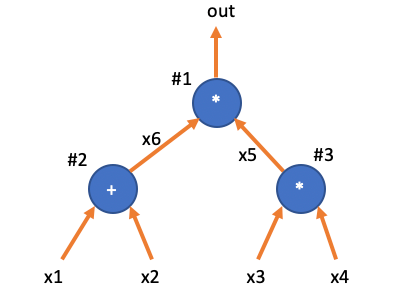
\includegraphics{img/img20230414202348.png}

下面是 \(Q\) 表格

$$
\begin{array}{c|c|c|c|cc}
i & q_L & q_R & q_M & q_C & q_O \\
\hline 0 & 0 & 0 & 0 & 99 & 1 \\
1 & 0 & 0 & 1 & 0 & 1 \\
2 & 1 & 1 & 0 & 0 & 1 \\
3 & 0 & 0 & 1 & 0 & 1
\end{array}
$$

下面是 \(S\) 表格,描述了哪些位置做了置换

\[
\begin{array}{c|c|c|c|}
i & \sigma_{a,i} & \sigma_{b,i} & \sigma_{c,i}  \\
\hline
0 & 0 & 4 & [9] \\
1 & \boxed{10} & \underline{11} & [8] \\
2 & 2 & 6 & \boxed{1} \\
3 & 3 & 7 & \underline{5} \\
\end{array}
\]

\hypertarget{ux5904ux7406-public-inputs}{%
\section{处理 Public Inputs}\label{ux5904ux7406-public-inputs}}

假如在上面给出的小电路中,要证明存在一个 Assignment,使得 out
的输入为一个特定的公开值,比如 \(out=99\)。最简单的办法是使用 \(Q\)
表中的 \(q_C\) 列,并增加一行约束,使得
\(q_L=q_R=q_M=0\),因此满足下面等式

\[
q_C(X) - q_O(X)w_c(X)  = 0
\]

但这个方案的问题是:这些公开值输入输出值被固定成了常数,如果公开值变化,那么
\(q_C(X)\) 多项式需要重新计算。如果整体上 \(W\)
表格的行数比较大,那么这个重新计算过程会带来很多的性能损失。

能否在表格中引入参数,以区分电路中的常数列?并且要求参数的变化并不影响其它电路的部分?这就需要再引入一个新的列,专门存放公开参数,记为
\(\phi\),因此,算术约束会变为:

\[
q_L(X)w_a(X)+q_R(X)w_b(X)+ q_M(X)w_a(X)w_b(X) - q_O(X)w_c(X)+q_C(X)+\phi(X) = 0
\]

我们还可以通过修改拷贝约束的方式引入公开参数。

\begin{quote}
{[}!TODO{]}
\end{quote}

\hypertarget{ux4f4dux7f6eux5411ux91cfux7684ux4f18ux5316}{%
\section{位置向量的优化}\label{ux4f4dux7f6eux5411ux91cfux7684ux4f18ux5316}}

我们上面在构造三个 \(\sigma\) 向量时,直接采用的自然数
\((0,1,2,\cdots)\),这样在协议开始前,Verifier 需要构造 3 个多项式
\(S_{id_a}(X),S_{id_b}(X),S_{id_c}(X)\),并且在协议最后一步查询
Oracle,获得三个多项式在挑战点 \(X=\zeta\) 处的取值
\((S_{id_a}(\zeta),S_{id_b}(\zeta),S_{id_c}(\zeta))\) 。

思考一下, \(\sigma\)
向量只需要用一些互不相等的值来标记置换即可,不一定要采用递增的自然数。如果我们采用
\(H=(1,\omega,\omega^2,\cdots)\) 的话,那么多项式 \({id_a}(X)\)
会被大大简化:

\[
\begin{split}
\vec{id}_a &= (1,\omega,\omega^2,\omega^3)\\
\vec{id}_b &= (k_1,k_1\omega,k_1\omega^2,k_1\omega^3)\\
\vec{id}_c &= (k_2,k_2\omega,k_2\omega^2,k_2\omega^3)\\
\end{split}
\]

其中 \(k_i\) 为互相不等的二次非剩余。

\[
{id_a}(X) = X, \quad {id_b}(X) = k_1\cdot X, \quad  {id_a}(X) = k_2\cdot X
\]

这样一来,这三个多项式被大大简化,它们在 \(X=\zeta\)
处的计算轻而易举,可以直接由 Verifier 完成。

这个小优化手段最早由 Vitalik 提出。采用 \(k_1\) 和 \(k_2\) 是为了产生
\((1,\omega,\omega^2,\omega^3)\) 的陪集(Coset),并保证 Coset
之间没有任何交集。我们前面提到 \(H=(1,\omega,\omega^2,\omega^3)\) 是
\(\mathbb{F}\) 的乘法子群,如果 \(H_1=k_1H\) 和 \(H_2=k_2H\)
存在交集,那么
\(H_1=H_2\)。这个论断可以简单证明如下:如果它们存在交集,那么
\(k_1\omega^i=k_2\omega^j\),于是 \(k_1=k_2\cdot\omega^{j-i}\),又因为
\(\omega^{j-i}\in H\),那么 \(k_1\in H_2\),那么
\(\forall i\in[N]. k_1\cdot \omega^i\in H_2\),那么
\(H_1\subset H_2\),同理可得 \(H_2\subset H_1\),于是 \(H_1=H_2\)。

如果 \(\sigma\) 的列数更多,那么我们需要选择多个 \(k_1, k_2,k_3,\ldots\)
且 \((k_i/k_j)^N\neq1\) 来产生不相交的 Coset。一种最直接的办法是采用
\(k_1,k_2,k_3,\ldots=g^1,g^2,g^3,\ldots\),其中 \(g\) 为乘法子群 \(T\)
的生成元, \(|T|*2^\lambda=p-1\)。

\hypertarget{ux534fux8baeux6846ux67b6}{%
\section{协议框架}\label{ux534fux8baeux6846ux67b6}}

预处理:Prover 和 Verifier 构造 \([q_L(X)]\), \([q_R(X)]\),
\([q_O(X)]\), \([q_M(X)]\), \([q_C(X)]\), \([{\sigma_a}(X)]\),
\([{\sigma_b}(X)]\), \([{\sigma_c}(X)]\)

第一步:Prover 针对 \(W\) 表格的每一列,构造 \([w_a(X)]\),
\([w_b(X)]\), \([w_c(X)]\), \(\phi(X)\) 使得

\[
q_L(X)w_a(X)+q_R(X)w_b(X)+ q_M(X)w_a(X)w_b(X) - q_O(X)w_c(X)+q_C(X) + \phi(X) = 0
\]

第二步: Verifier 发送随机数 \(\beta\) 与 \(\gamma\);

第三步:Prover 构造 \([z(X)]\),使得

\[
\begin{split}
L_0(X)(z(X)-1) &= 0 \\
z(\omega\cdot X)g(X) -  z(X)f(X) &=0
\end{split}
\]

第四步:Verifier 发送随机挑战数 \(\alpha\);

第五步:Prover 计算 \(h(X)\),并构造商多项式 \([t(X)]\)

\[
\begin{split}
h(X) = &\ q_L(X)w_a(X)+q_R(X)w_b(X)+ q_M(X)w_a(X)w_b(X) - q_O(X)w_c(X)+q_C(X) + \phi(X) \\
 & + \alpha(z(\omega X)\cdot g(X)-z(X)\cdot f(X)) + \alpha^2(L_0(X)\cdot(z(X)-1))
\end{split}
\]

其中

\[
\begin{split}
f(X)&=\Big(w_a(X)+\beta\cdot {id_a}(X)+\gamma\Big)\Big(w_b(X)+\beta\cdot {id_b}(X)+\gamma\Big)\Big(w_c(X)+\beta\cdot {id_c}(X)+\gamma\Big)\\
g(X)&=\Big(w_a(X)+\beta\cdot {\sigma_a}(X)+\gamma\Big)\Big(w_b(X)+\beta\cdot {\sigma_b}(X)+\gamma\Big)\Big(w_c(X)+\beta\cdot {\sigma_c}(X)+\gamma\Big)\\
\end{split}
\]

其中商多项式 \(t(X)=\frac{h(X)}{z_H(X)}\) ;

第六步:Verifier 发送随机挑战数 \(\zeta\),查询上述的所有 Oracle,得到 -
\(\bar{w}_a=w_a(\zeta)\), \(\bar{w}_b=w_b(\zeta)\),
\(\bar{w}_c=w_c(\zeta)\) - \(\bar{q}_L=q_L(\zeta)\),
\(\bar{q}_R=q_R(\zeta)\), \(\bar{q}_M=q_M(\zeta)\),
\(\bar{q}_O=q_O(\zeta)\), \(\bar{q}_C=q_C(\zeta)\) -
\(\bar{\sigma}_a=\sigma_a(\zeta)\),
\(\bar{\sigma}_b=\sigma_b(\zeta)\), \(\bar{\sigma}_c=\sigma_c(\zeta)\)
- \(\bar{z}\_{(\omega\cdot\zeta)}=z(\omega\cdot\zeta)\),
\(\bar{z}_{(\zeta)}=z(\zeta)\) - \(\bar{t}=t(\zeta)\)

Verifier 还要自行计算 -
\(\bar{f}_{(\zeta)} =(\bar{w}_a+\beta\cdot \zeta + \gamma) (\bar{w}_b+\beta\cdot k_1\cdot \zeta +\gamma)(\bar{w}_c+\beta\cdot k_2 \cdot \zeta +\gamma)\)
-
\(\bar{g}_{(\zeta)}=(\bar{w}_a+\beta\cdot \bar{\sigma}_1 + \gamma) (\bar{w}_b+\beta\cdot\bar{\sigma}_2+\gamma)(\bar{w}_c+\beta\cdot\bar{\sigma}_3+\gamma)\)
- \(L_0(\zeta)\) - \(z_H(\zeta)\) - \(\phi(\zeta)\)

验证步:

\[
\begin{split}
& \bar{q}_L\bar{w}_a+\bar{q}_R\bar{w}_b+ \bar{q}_M\bar{w}_a\bar{w}_b - \bar{q}_O\bar{w}_c+\bar{q}_C + \phi(\zeta)  \\
& \qquad \qquad + \alpha(\bar{z}\_{(\omega\cdot\zeta)}\cdot \bar{g}\_{(\zeta)}-\bar{z}\_{(\zeta)}\cdot \bar{f}\_{(\zeta)})+ \alpha^2(L_0(\zeta)\cdot(\bar{z}\_{(\zeta)}-1))\overset{?}{=}\bar{t}\cdot z_H(\zeta)
\end{split}
\]


\hypertarget{ux7406ux89e3-plonkux4e94ux591aux9879ux5f0fux627fux8bfa}{%
\chapter{多项式承诺}\label{ux7406ux89e3-plonkux4e94ux591aux9879ux5f0fux627fux8bfa}}

\hypertarget{ux4ec0ux4e48ux662fux591aux9879ux5f0fux627fux8bfa}{%
\section{什么是多项式承诺}\label{ux4ec0ux4e48ux662fux591aux9879ux5f0fux627fux8bfa}}

所谓承诺,是对消息「锁定」,得到一个锁定值。这个值被称为对象的「承诺」。

\[
c = commit(x)
\]

这个值和原对象存在两个关系,即 Hiding 与 Binding。

Hiding: \(c\) 不暴露任何关于 \(x\) 的信息;

Binding:难以找到一个 \(x', x'\neq x\),使得 \(c=commit(x')\)。

最简单的承诺操作就是 Hash 运算。请注意这里的 Hash
运算需要具备密码学安全强度,比如 SHA256, Keccak 等。除了 Hash
算法之外,还有 Pedersen 承诺等。

顾名思义,多项式承诺可以理解为「多项式」的「承诺」。如果我们把一个多项式表达成如下的公式,

\[
f(X) = a_0 + a_1X + a_2X^2 + \cdots + a_nX^n
\]

那么我们可以用所有系数构成的向量来唯一标识多项式 \(f(X)\)。

\[
(a_0, a_1, a_2,\ldots, a_n)
\]

如何对一个多项式进行承诺?很容易能想到,我们可以把「系数向量」进行 Hash
运算,得到一个数值,就能建立与这个多项式之间唯一的绑定关系。

\[
C_1 = \textrm{SHA256}(a_0\parallel a_1 \parallel a_2 \parallel \cdots \parallel a_n)
\]

或者,我们也可以使用 Petersen 承诺,通过一组随机选择的基,来计算一个 ECC
点:

\[
C_2 = a_0 G_0 + a_1  G_1 + \cdots + a_n G_n
\]

如果在 Prover 承诺多项式之后,Verifier
可以根据这个承诺,对被锁定的多项式进行求值,并希望 Prover
可以证明求值的正确性。假设 \(C=Commit(f(X))\),Verifier 可以向提供承诺的
Prover 询问多项式在 \(X=\zeta\) 处的取值。Prover
除了回复一个计算结果之外(如 \(f(\zeta) = y\)) ,还能提供一个证明
\(\pi\),证明 \(C\) 所对应的多项式 \(f(X)\) 在 \(X=\zeta\) 处的取值
\(y\) 的正确性。

多项式承诺的这个「携带证明的求值」特性非常有用,它可以被看成是一种轻量级的「可验证计算」。即
Verifier 需要把多项式 \(f(X)\)
的运算代理给一个远程的机器(Prover),然后验证计算(计算量要小于直接计算\(f(X)\))结果
\(y\)
的正确性;多项式承诺还能用来证明秘密数据(来自Prover)的性质,比如满足某个多项式,Prover
可以在不泄漏隐私的情况下向 Verifier 证明这个性质。

虽然这种可验证计算只是局限在多项式运算上,而非通用计算。但通用计算可以通过各种方式转换成多项式计算,从而依托多项式承诺来最终实现通用的可验证计算。

按上面 \(C_2\) 的方式对多项式的系数进行 Pedersen 承诺,我们仍然可以利用
Bulletproof-IPA
协议来实现求值证明,进而实现另一种多项式承诺方案。此外,还有 KZG10
方案,FRI,Dark,Dory 等等其它方案。

\hypertarget{kzg10-ux6784ux9020}{%
\section{KZG10 构造}\label{kzg10-ux6784ux9020}}

与 Pedersen 承诺中用的随机基向量相比,KZG10
多项式承诺需要用一组具有内部代数结构的基向量来代替。

\[
(G_0, G_1, G_2, \ldots, G_{d-1}, H_0, H_1) = (G, \chi G, \chi^2G, \ldots, \chi^{d-1}G, H, \chi H)
\]

请注意,这里的 \(\chi\) 是一个可信第三方提供的随机数,也被称为
Trapdoor,需要在第三方完成 Setup 后被彻底删除。它既不能让 Verifier
知道,也不能让 Prover 知道。当 \(\vec{G}\) 设置好之后, \(\chi\)
被埋入了基向量中。这样一来,从外部看,这组基向量与随机基向量难以被区分。其中
\(G\in\mathbb{G}_1\),而 \(H\in\mathbb{G}_2\),并且存在双线性映射
\(e\in \mathbb{G}_1\times\mathbb{G}_2\to \mathbb{G}_T\)。

对于一个多项式 \(f(X)\) 进行 KZG10 承诺,也是对其系数向量进行承诺:

\[
\begin{split}
C_{f(X)} &= a_0 G_0 + a_1  G_1 + \cdots + a_{n-1} G_{n-1} \\
 & = a_0  G + a_1 \chi G + \cdots + a_{n-1}\chi^{n-1} G\\
 & = f(\chi) G
\end{split}
\]

这样承诺 \(C_{f(X)}\) 巧好等于 \(f(\chi) G\)。

对于双线性群,我们下面使用 Groth 发明的符号 \([1]_1\triangleq G\),
\([1]_2\triangleq H\) 表示两个群上的生成元,这样 KZG10
的系统参数(也被称为 SRS, Structured Reference String)可以表示如下:

\[
\mathsf{srs}=([1]_1,[\chi]_1,[\chi^2]_1,[\chi^3]_1,\ldots,[\chi^{n-1}]_1,[1]_2,[\chi]_2)
\]

而 \(C_{f(X)}=[f(\chi)]_1\)。

下面构造一个 \(f(\zeta) = y\) 的 Open
证明。根据多项式余数定理,我们可以得到下面的等式:

\[
f(X) = q(X)\cdot (X-\zeta) + y
\]

这个等式可以解释为,任何一个多项式都可以除以另一个多项式,得到一个商多项式加上一个余数多项式。由于多项式在
\(X=\zeta\) 处的取值为 \(y\),那么我们可以确定:余数多项式一定为 \(y\)
,因为等式右边的第一项在 \(X=\zeta\) 处取值为零。所以,如果
\(f(\zeta)=y\),我们可以断定: \(g(X) = f(X)-y\) 在 \(X=\zeta\)
处等零,所以 \(\zeta\) 为 \(g(X)\) 的根,于是 \(g(X)\) 一定可以被
\((X-\zeta)\) 这个不可约多项式整除,即一定\textbf{存在}一个商多项式
\(q(X)\),满足上述等式。

而 Prover 则可以提供 \(q(X)\) 多项式的承诺,记为 \(C_q\),作为
\(f(\zeta)=y\) 的证明,Verifier 可以检查 \([q(\chi)]\)
是否满足整除性来验证证明。因为如果 \(f(\zeta)\neq y\),那么 \(g(X)\)
则无法被 \((X-\zeta)\) 整除,即使 Prover
提供的承诺将无法通过整除性检查:

\[
(f(X)-y)\cdot 1 \overset{?}{=} q(X) \cdot (X-x)
\]

承诺 \(C_{f(X)}\) 是群 \(\mathbb{G}_1\)
上的一个元素,通过承诺的加法同态映射关系,以及双线性映射关系
\(e\in \mathbb{G}_1\times\mathbb{G}_2\to \mathbb{G}_T\),Verifier 可以在
\(\mathbb{G}_T\) 上验证整除性关系:

\[
e(C\_{f(X)} - y[1]_1, [1]_2) \overset{?}{=} e(C\_{q(X)}, [\chi]_2 - \zeta [1]_2)
\]

有时为了减少 Verifier 在 \(\mathbb{G}_2\)
上的昂贵操作,上面的验证等式可以变形为:

\[
f(X) + \zeta\cdot q(X) - y =  q(X)\cdot X
\]

\[
e(C\_{f(X)} + \zeta\cdot C\_{q(X)} -y, [1]_2)\overset{?}{=} e(C\_{q(X)}, [\chi]_2)
\]

\hypertarget{ux540cux70b9-open-ux7684ux8bc1ux660eux805aux5408}{%
\section{同点 Open
的证明聚合}\label{ux540cux70b9-open-ux7684ux8bc1ux660eux805aux5408}}

在一个更大的安全协议中,假如同时使用多个多项式承诺,那么他们的 Open
操作可以合并在一起完成。即把多个多项式先合并成一个更大的多项式,然后仅通过
Open 一点,来完成对原始多项式的批量验证。

假设我们有多个多项式, \(f_1(X)\), \(f_2(X)\),Prover 要同时向 Verifier
证明 \(f_1(\zeta)=y_1\) 和 \(f_2(\zeta)=y_2\),那么有

\[
\begin{array}{l}
f_1(X) = q_1(X)\cdot (X-\zeta) + y_1\\ 
f_2(X) = q_2(X) \cdot (X-\zeta) + y_2 \\
\end{array}
\]

通过一个随机数 \(\nu\),Prover 可以把两个多项式 \(f_1(X)\) 与 \(f_2(X)\)
折叠在一起,得到一个临时的多项式 \(g(X)\) :

\[
g(X) = f_1(X) + \nu\cdot f_2(X)
\]

进而我们可以根据多项式余数定理,推导验证下面的等式:

\[
g(X) - (y_1 + \nu\cdot y_2) = (X-\zeta)\cdot (q_1(X) + \nu\cdot q_2(X))
\]

我们把等号右边的第二项看作为「商多项式」,记为 \(q(X)\):

\[
q(X) = q_1(X) + \nu\cdot q_2(X)
\]

假如 \(f_1(X)\) 在 \(X=\zeta\) 处的求值证明为 \(\pi_1\),而 \(f_2(X)\)
在 \(X=\zeta\) 处的求值证明为 \(\pi_2\),那么根据群加法的同态性,Prover
可以得到商多项式 \(q(X)\) 的承诺:

\[
[q(\chi)]_1 = \pi = \pi_1 + \nu\cdot\pi_2
\]

因此,只要 Verifier 发给 Prover 一个额外的随机数
\(\nu\),双方就可以把两个(甚至多个)多项式承诺折叠成一个多项式承诺
\(C_g\):

\[
C_g = C_1 + \nu\ast C_2
\]

并用这个折叠后的 \(C_g\) 来验证多个多项式在一个点处的运算取值:

\[
y_g = y_1 + \nu\cdot y_2
\]

从而把多个求值证明相应地折叠成一个,Verifier 可以一次验证完毕:

\[
e(C-y\ast G_0, H_0) \overset{?}{=}e(\pi, H_1 - x\ast H_0)
\]

由于引入了随机数
\(\nu\),因此多项式的合并不会影响承诺的绑定关系(Schwartz-Zippel
定理)。

\hypertarget{ux534fux8bae}{%
\subsection{协议:}\label{ux534fux8bae}}

公共输入: \(C\_{f_1}=[f_1(\chi)]_1\), \(C\_{f_2}=[f_2(\chi)]_1\),
\(\zeta\), \(y_1\), \(y_2\)

私有输入: \(f_1(X)\), \(f_2(X)\)

证明目标: \(f_1(\zeta)=y_1\), \(f_2(\zeta)=y_2\)

第一轮:Verifier 提出挑战数 \(\nu\)

第二轮:Prover 计算 \(q(X)=f_1(X)+\nu\cdot f_2(X)\),并发送
\(\pi=[q(\chi)]_1\)

第三轮:Verifier 计算 \(C_g=C_{f_1} + \nu\cdot C_{f_2}\),
\(y_g = y_1 + \nu\cdot y_2\)

\[
e(C_g - [y_g]_1, [1]_2)\overset{?}{=}e(\pi, [\chi-\zeta]_2)
\]

\hypertarget{ux591aux9879ux5f0fux7ea6ux675fux4e0eux7ebfux6027ux5316}{%
\section{多项式约束与线性化}\label{ux591aux9879ux5f0fux7ea6ux675fux4e0eux7ebfux6027ux5316}}

假设 \([f(\chi)]_1, [g(\chi)]_1, [h(\chi)]_1\) 分别是 \(f(X),g(X),h(X)\)
的 KZG10 承诺,如果 Verifier 要验证下面的多项式约束:

\[
f(X) + g(X) \overset{?}{=} h(X)
\]

那么 Verifier 只需要把前两者的承诺相加,然后判断是否等于 \([h(\chi)]_1\)
即可

\[
[f(\chi)]_1 + [g(\chi)]_1 \overset{?}{=} [h(\chi)]_1
\]

如果 Verifier 需要验证的多项式关系涉及到乘法,比如:

\[
f(X) \cdot g(X) \overset{?}{=} h(X)
\]

最直接的方法是利用双线性群的特性,在 \(\mathbb{G}_T\)
上检查乘法关系,即验证下面的等式:

\[
e([f(\chi)]_1, [g(\chi)]_2) \overset{?}{=} e([h(\chi)]_1, [1]_2)
\]

但是如果 Verifier 只有 \(g(X)\) 在 \(\mathbb{G}_1\) 上的承诺
\([g(\chi)]_1\),而非是在 \(\mathbb{G}_2\) 上的承诺
\([g(\chi)]_2\),那么Verifer 就无法利用双线性配对操作来完成乘法检验。

另一个直接的方案是把三个多项式在同一个挑战点 \(X=\zeta\)
上打开,然后验证打开值之间的关系是否满足乘法约束:

\[
f(\zeta)\cdot g(\zeta)\overset{?}{=} h(\zeta)
\]

同时 Prover 还要提供三个多项式求值的证明
\((\pi_{f(\zeta)},\pi_{g(\zeta)},\pi_{h(\zeta)})\) 供 Verifier 验证。

这个方案的优势在于多项式的约束关系可以更加复杂和灵活,比如验证下面的稍微复杂些的多项式约束:

\[
f_1(X)f_2(X) + h_1(X)h_2(X)h_3(X) + g(X) = 0
\]

假设 Verifier 已拥有这些多项式的 KZG10 承诺, \([f_1(\chi)]_1\),
\([f_2(\chi)]_1\), \([h_1(\chi)]_1\), \([h_2(\chi)]_1\),
\([h_3(\chi)]_1\), \([g(\chi)]_1\)。最直接粗暴的方案是让 Prover
在挑战点 \(X=\zeta\) 处打开这 6 个承诺,发送 6 个 Open
值和对应的求值证明:

\[
(f_1(\zeta),\pi_{f_1}),(f_2(\zeta),\pi_{f_2}),(h_1(\zeta),\pi_{h_1}),(h_2(\zeta),\pi_{h_2}),(h_3(\zeta),\pi_{h_3}),(g(\zeta),\pi_{g})
\]

Verifier 验证 \(6\) 个求值证明,并且验证多项式约束:

\[
f_1(\zeta)f_2(\zeta) + h_1(\zeta)h_2(\zeta)h_3(\zeta) + g(\zeta) \overset{?}{=} 0
\]

我们可以进一步优化,比如考虑对于 \(f(X) \cdot g(X) = h(X)\)
这样一个简单的多项式约束,Prover 可以减少 Open 的数量。比如 Prover 先
Open \(\bar{f} = f(\zeta)\),发送求值证明 \(\pi\_{f(\zeta)}\)
然后引入一个辅助多项式 \(L(X)= \bar{f}\cdot g(X)-h(X)\),再 Open
\(L(X)\) 在 \(X=\zeta\) 处的取值。

显然对于一个诚实的 Prover, \(L(\zeta)\) 求值应该等于零。对于
Verifier,它在收到 \(\bar{f}\)
之后,就可以利用承诺的加法同态性,直接构造 \(L(X)\) 的承诺:

\[
[L(\chi)]_1 = \bar{f}\cdot [g(\chi)]_1 - [h(\chi)]_1
\]

这样一来,Verifier 就不需要单独让 Prover 发送 \(L(X)\) 的
Opening,也不需要发送新多项式 \(L(X)\) 的承诺。Verifier 然后就可以验证
\(f(X) \cdot g(X) = h(X)\) 这个多项式约束关系:

\[
e([L(\chi)]_1, [1]_2)\overset{?}{=} e(\pi\_{L(\zeta)}, [\chi-\zeta]_2)
\]

这个优化过后的方案,Prover 只需要 Open 两次。第一个 Opening 为
\(\bar{f}\),第二个 Opening 为 \(0\)。而后者是个常数,不需要发送给
Verifier。Prover
只需要发送两个求值证明,不过我们仍然可以用上一节提供的聚合证明的方法,通过一个挑战数
\(\nu\),Prover 可以聚合两个多项式承诺,然后仅需要发送一个求值证明。

我们下面尝试优化下 \(6\) 个多项式的约束关系的协议:
\(f_1(X)f_2(X) + h_1(X)h_2(X)h_3(X) + g(X) = 0\)。

\hypertarget{ux534fux8bae-1}{%
\subsection{协议:}\label{ux534fux8bae-1}}

公共输入: \(C\_{f_1}=[f_1(\chi)]_1\), \(C\_{f_2}=[f_2(\chi)]_1\),
\(C\_{h_1}=[h_1(\chi)]_1\), \(C\_{h_2}=[h_2(\chi)]_1\),
\(C\_{h_3}=[h_3(\chi)]_1\), \(C\_{g}=[g(\chi)]_1\),

私有输入: \(f_1(X)\), \(f_2(X)\), \(h_1(X)\), \(h_2(X)\),
\(h_3(X)\), \(g(X)\)

证明目标: \(f_1(X)f_2(X) + h_1(X)h_2(X)h_3(X) + g(X) = 0\)

第一轮:Verifier 发送 \(X=\zeta\)

第二轮:Prover 计算并发送三个Opening, \(\bar{f_1}=f_1(\zeta)\),
\(\bar{h}_1=h_1(\zeta)\), \(\bar{h}_2=h_2(\zeta)\),

第三轮:Verifier 发送 \(\nu\) 随机数

第四轮:Prover 计算 \(L(X)\) ,利用 \(\nu\) 折叠
\((L(X), f_1(X),h_1(X),h_2(X))\) 这四个承诺,并计算商多项式
\(q(X)\),发送其承诺 \([q(\chi)]_1\) 作为折叠后的多项式在 \(X=\zeta\)
处的求值证明

\[
L(X)=\bar{f}_1\cdot f_2(X) + \bar{h}_1\bar{h}_2\cdot h_3(X) + g(X)
\]

\[
q(X)=\frac{1}{X-\zeta}\Big(L(X) + \nu\cdot (f_1(X)-\bar{f}_1)+\nu^2\cdot (h_1(X)-\bar{h}_1)+\nu^3\cdot (h_2(X)-\bar{h}_2)\Big)
\]

第五轮:Verifier 计算辅助多项式 \(L(X)\) 的承诺 \([L]_1\):

\[
[L]_1 = \bar{f}_1\cdot[f_2(\chi)]_1 + \bar{h}_1\bar{h}_2\cdot[h_3(\chi)]_1 + [g(\chi)]_1
\]

计算折叠后的多项式的承诺:

\[
[F]_1=[L]_1 + \nu \cdot  [f_1(\chi)]_1+\nu^2[h_1(\chi)]_1+\nu^3[h_2(\chi)]_1
\]

计算折叠后的多项式在 \(X=\zeta\) 处的求值:

\[
E=\nu\cdot \bar{f}_1 + \nu^2\cdot\bar{h}_1+ \nu^3\cdot\bar{h}_2
\]

检查下面的验证等式:

\[
e([F]_1-[E]_1 + \zeta[q(\chi)]_1, [1]_2)\overset{?}{=}e([q(\chi)]_1, [\chi]_2)
\]

这个优化后的协议,Prover 仅需要发送三个
Opening,一个求值证明;相比原始方案的 6 个 Opening和 6
个求值证明,大大减小了通信量(即证明大小)。





\hypertarget{ux7406ux89e3-plonkux516dux5b9eux73b0-zero-knowledge}{%
\chapter{实现 Zero Knowledge}\label{ux7406ux89e3-plonkux516dux5b9eux73b0-zero-knowledge}}

在前文的 Plonk
协议中,所有的多项式承诺都没有混入额外的随机数进行保护,因此当一个未被随机化的多
项式承诺 \(f(X)\) 经过一次或者多次 Open,会泄露 \(f(X)\)
自身的信息,这会限制协议在需要隐私保护的 场景中应用。

考虑一个 \(3\) 次多项式 \(f(X)\),只要它在四个不同的点上 Open
,多项式就可以通过 Lagrange 插值来复原。
然而即使一个次数超过一百万的多项式,哪怕被打开一次也会泄漏关于原多项式的部分信息。

为了实现 Zero Knowledge 性质的
Plonk,我们需要在多项式中加入足够多的随机因子,确保在多项式 打开 \(k\)
次之后,仍然不会泄漏原多项式的信息,保证没有知识泄漏。

Plonk 协议的大致流程为:Prover 构造多项式,然后发送多项式的承诺给
Verifier。然后 Verfier 挑战两个随机挑战点 \(X=\zeta\) 与
\(X=\omega\cdot \zeta\),其中 \(\omega\) 为 子群 \(H\) 的生成元。下面是
Prover 需要构造的多项式列表:

\begin{itemize}
\item
  Witness 多项式: \(w_a(X), w_b(X), w_c(X)\)
\item
  置换累乘多项式: \(z(X)\)
\item
  商多项式: \(t_{low}(X)\), \(t_{mid}(X)\), \(t_{high}(X)\)
\end{itemize}

其中三个 Witness 多项式要在 \(X=\zeta\) 这一个点处打开,置换累乘多项式
\(z(X)\) 要在 \(X=\zeta\), \(X=\omega\cdot\zeta\)
两个点处打开,而三个商多项式则不需要被打开。

Prover 要混入两类随机因子,第一类是保护承诺本身,满足信息隐藏
Hiding,一个承诺一般只需要混入一个随机数即可;
第二类是保护多项式承诺在打开之后仍然保证原多项式信息不会泄漏。如果多项式打开的次数越多(假设每次打开的位置都不同),
Prover 就要混入越多的随机因子。

第一类的随机因子,也可以用多项式承诺方案来实现,比如
Bulletproof-IPA,或者 KZG10-with-Hiding,这些多项式承诺方案本身已经支持
Hiding 。如果 Plonk 后端采用的是朴素的 KZG10,那么就需要在 Plonk
协议层面增加足够的随机因子,不仅保证承诺自身的 Hiding
性质,还要保护承诺的打开。

下面我们介绍两个不同的混入随机因子方案实现 Zero Knowledge
的方法。第一个方法比较经典,是为多项式加上一个盲化(Blinding)用途的多项式,\cite{Plonk}
论文(或其它学术论文)中正是采用的这种方法。而第二个方法是在向量的对齐填充空间里面填入随机数,再插值产生多项式的,这是工程实现中的常见方法。

\hypertarget{ux65b9ux6cd5ux4e00blinding-ux591aux9879ux5f0f}{%
\section{方法一:Blinding
多项式}\label{ux65b9ux6cd5ux4e00blinding-ux591aux9879ux5f0f}}

我们先看 Witness 多项式 \(w_a(X)\),它是由下面的等式计算:

\[
w_a(X)=w_{a,0}L_0(X) + w_{a,1}L_1(X) + w_{a,2}L_2(X) + \cdots + w_{a,n-1}L_{n-1}(X)
\]

我们假设 \(n\leq N\),其中 \(N=|H|\)。

在 Plonk 协议中,Prover 需要计算 \(w_a(\zeta)\) 的取值,其中 \(\zeta\)
为 Verifier 给出的随机挑战点。

如果我们直接鲁莽地在 \(w_a(X)\) 中混入随机数 \(b_0\),比如
\(w'_{a}(X)=w_a(X) + b_0\),那么 \(w_a'(X)\) 可能就不再满足算术约束:

\[
q_L(X)w'_a(X)+q_R(X)w_b(X)+ q_M(X)w_a(X)w_b(X) - q_O(X)w_c(X)+q_C(X) + \phi(X) \neq t(X)\cdot z_H(X)
\]

而且也无法满足置换约束。

如果要让随机化后的多项式 \(w'_a(X)\)
满足「算术约束」和「置换约束」,那么我们可以考虑在乘法子群 \(H\)
之外增加一些随机的点,这样可以让随机化后的多项式 \(w'_a(X)\) 在 \(H\)
整个乘法子群上的取值仍然与 \(w_a(X)\)
完全相等,但是整个多项式却已经被随机化了。所谓的在 \(H\)
上的取值相等,就是保证随机化后的多项式仍然可以被 \(z_H(X)\)
整除。下面是随机化多项式的构造:

\[
w'_a(X) = (b_1 X + b_0)\cdot z_H(X) + w_a(X)
\]

这里 \(b_1X+b_0\) 为 Blinding 多项式,包含两个随机因子
\((b_0, b_1)\),它们恰好是自变量的不同次数的系数,这样可以保证线性不相关。换个方式理解,只有对这个
Blinding
多项式打开两次以上,才可以计算出所有的随机因子。如果只打开一次,Blinding
多项式会被消耗掉一个随机因子,还剩下一个起作用的随机因子。

简单检查下,我们可以发现新定义的 \(w'_a(X)\)
符合要求,能满足算术约束。同时因为
\(w'_a(X)=w_a(X),\forall x\in H\),因此 \(w'_a(X)\) 也一定满足置换关系。

这里 \(w'_a(X)\) 被混入了两个随机因子,其中一个随机因子可以保护
\([w'_a(x)]\) 被打开一次,另一个随机因子用来实现承诺 \([w'_a(x)]\)
本身的信息隐藏。

考虑下置换累乘多项式 \(z(X)\),假如多项式承诺 \([z(X)]\)
被打开两次的话,那么就需要混入三个随机因子,构造一个次数为 \(2\) 的
Blinder 多项式, \(b_0 + b_1 X + b_2X^2\),然后混入到 \(z(X)\) 中:

\[
z'(X) = (b_0 + b_1X+ b_2X^2)\cdot z_H(X) + z(X)
\]

最后考虑商多项式 \(t_{low}(X)\), \(t_{mid}(X)\),
\(t_{high}(X)\),由于他们不需要在任何点打开,因此只要加上随机因子即可,不过这几个商多项式有额外的要求,即他们三个需要一起能拼出真正的商多项式
\(t(X)\):

\[
t(X) = t_{low}(X) + t_{mid}(X)\cdot X^N + t_{high}(X)\cdot X^{2N}
\]

我们可以采用下面的方式,为每一个多项式分片混入一个随机因子,并且保证他们拼起来之后仍然等于
\(t(X)\):

\[
\begin{split}
t'\_{low}(X)&=t\_{low}(X) + b_0X^N\\
t'\_{mid}(X)&=t\_{mid}(X) - b_0 + b_1X^N\\
t'\_{high}(X)&=t\_{high}(X) - b_1\\
\end{split}
\]

容易检验:

\[
\begin{split}
&t'\_{low}(X) + t'\_{mid}(X)\cdot X^N + t'\_{high}(X)\cdot X^{2N} \\
=\ &  t\_{low}(X) + b_0X^N + (t\_{mid}(X) - b_0 + b_1X^N)\cdot X^N + (t\_{high}(X) - b_1)\cdot X^{2n} \\
=\ & t\_{low}(X) + t\_{mid}(X)\cdot X^N + t\_{high}(X)\cdot X^{2N} \\
=\ & t(X)
\end{split}
\]

同理,如果 \(t(X)\) 的次数达到了 \(4N\),那么就需要三个随机数给四个
\(t(X)\) 分段加上随机数,实现 Hiding。

这个方法存在一个问题,就是 Blinding 多项式的次数会超过 \(N\) ,这里
\(N=|H|\)。因为 \(z_H(X)\) 的次数为 \(N\),因此
\((b_1 X + b_0)\cdot z_H(X)\) 次数为 \(N+1\)。如果 Plonk 后端采用的是
Bulletproof-IPA 这类的多项式承诺,承诺会要求多项式的次数按 \(2^k\)
对齐,这样盲化之后的多项式的次数刚刚超出 \(N\),只能对齐到 \(2N\)。一些
Plonk 变种协议可能会把 Witness table
的列数增加,稍稍超出的多项式次数会使 \(t(X)\)
的计算在一个更大的子群上完成。

\hypertarget{ux65b9ux6cd5ux4e8cux968fux673aux56e0ux5b50ux5bf9ux9f50}{%
\section{方法二:随机因子对齐}\label{ux65b9ux6cd5ux4e8cux968fux673aux56e0ux5b50ux5bf9ux9f50}}

下面介绍的第二种方法不会推高多项式的次数。考虑到 \(H\) 子群的大小 \(N\)
是按 \(2^k\) 对齐,在实际电路中,一般情况下需要把 Witness Table
的长度对齐到 \(N\),为了对齐,需要把空余的空间用零填满。

那么这里可以用随机数来代替零填充对齐空间,好处是这些随机数可以保护表中的其它正常数据。

Daniel Lubarov 按照这个思路给出了第二种随机数填充实现 Zero-Knowledge
性质的办法 \footnote{Adding zero knowledge to Plonk-Halo \url{https://mirprotocol.org/blog/Adding-zero-knowledge-to-Plonk-Halo}}

对于商多项式,因为方法一不会推高他们的次数,因此我们下面只考虑剩下的两类多项式:

\begin{itemize}
\item
  Witness 多项式: \(w_a(X), w_b(X), w_c(X)\)
\item
  置换累乘多项式: \(z(X)\)
\end{itemize}

先看第一类多项式,以 \(w_a(X)\) 为例,它编码了 \(w_{a,i}\)
向量。如果本身向量长度不足
\(N\),一般情况下是用零补齐,我们现在可以考虑让 Prover
额外用两个随机数补齐,这样做的效果和方法一的 Blinding 多项式完全一样。
如下所示:

\[
w'_a(X) = w_a(X) + (b_0\cdot L\_{N-2}(X) + b_1\cdot L\_{N-1}(X))
\]

其中 \(b(X)=b_0\cdot L_{N-2}(X) + b_1\cdot L_{N-1}(X)\) 也可以看成是利用
Lagrange Basis 产生的 Blinding 多项式。这里假设 \(\{w_{a,i}\}\) 的长度为
\(N-2\), \((b_0, b_1)\) 为两个随机数。假设 \(w_a(X)\)
的系数为固定值,那么当 \(w'\_a(X)\) 被打开两次之后,
\(b(X)=b_0\cdot L\_{N-2}(X) + b_1\cdot L\_{N-1}(X)\)
的系数即可被求解,从而失去随机化的能力。因此, \(w'_a(X)\)
只能承受一次安全的打开操作(假设协议基于 Non-hiding 的多项式承诺)。

对于置换累乘多项式 \(z(X)\),则需要在累乘向量 \(\vec{z}\)
的尾部引入随机值。考虑下 \(\vec{z}\) 的计算方式:

\[
z_{i+1} = z_i\cdot \frac{(w_a(X) + \beta\cdot X+\gamma)(w_b(X) + \beta\cdot k_1X+\gamma)(w_a(X) + \beta\cdot k_2X+\gamma)}{(w_a(X) + \beta\cdot\sigma_a(X)+\gamma)(w_b(X) + \beta\cdot \sigma_b(X)+\gamma)(w_a(X) + \beta\cdot\sigma_c(X)+\gamma)}
\]

列出所有的 \(z_i\) 的计算如下:

\[
\begin{array}{|c|c|c|}
i & H_i & z_i\\
\hline
0 & \omega^0=1 & 1\\
1 & \omega^1 & 1\cdot \frac{f_0}{g_0}\\
2 & \omega^2 & \frac{f_0}{g_0}\cdot \frac{f_1}{g_1}\\
3 & \omega^3 & \frac{f_0f_1}{g_0g_1}\cdot \frac{f_2}{g_2}\\
\vdots & & \vdots\\
N-2 & \omega^{N-2} & \frac{f_0f_1\cdots f_{N-4}}{g_0g_1\cdots g_{N-4}}\cdot \frac{f_{N-3}}{g_{N-3}} \\
N-1 & \omega^{N-1} & \frac{f_0f_1\cdots f_{N-3}}{g_0g_1\cdots g_{N-3}}\cdot \frac{f_{N-2}}{g_{N-2}} \\
N & \omega^{N}=1 & \frac{f_0f_1\cdots f_{N-1}}{g_0g_1\cdots g_{N-1}}  = 1
\end{array}
\]

假如我们想设置 \(z_{N-1}\) 为随机值,我们需要让 \(w_{a,N-1}\) 和
\(w_{a,N-2}\) 这两个元素设置一个 Copy Constraint,并填上同一个随机数
\(\rho_1\)。如果 \(w_{b,N-1}\) 和 \(w_{b,N-2}\) 设置为零,那么

\[
\frac{f_{N-2}}{g_{N-2}} = \frac{(\rho_1 + \beta \cdot \omega^{N-2} + \gamma)}{(\rho_1 + \beta \cdot \omega^{N-1}+ \gamma)}
\]

又因为

\[
z_{N-1} = z_{N-2}\cdot \frac{f_{N-2}}{g_{N-2}}
\]

那么 \(z_{N-1}\) 的概率分布与\(\rho_1\) 相同。这样我们通过把 Witness
Table 的最后两行用来填入随机数 \(\rho_1\),并且设置一个 Copy Constraint
来随机化 \(z_{N-1}\)。如果要再引入一个随机数
\(\rho_2\),一种方法是我们再征用 Witness table 的两行,
\(i=N-4, N-3\),可以让 \(z_{N-4}\) 随机化。或者我们节省下空间,利用
\(w_{b,N-3}\) 与 \(w_{b,N-2}\) 来构造一个随机数 \(\rho_2\) 的 Copy
Constraint。同理,我们可以再用两行 \(i=N-4, N-3\) 来引入 \(\rho_3\)。
这样,我们总共征用了四行,引入了三个随机数 \(\rho_1,\rho_2,\rho_3\):

\[
\begin{array}{c|c|c|c|}
i & w_a & w_b & w_c \\
\hline
0 & \cdots & \cdots & \cdots \\
\vdots & \vdots & \vdots & \vdots \\
N-4 & {\color{green}\rho_3} & 0& 0\\
N-3 & {\color{green}\rho_3} & {\color{blue}\rho_2} & 0\\
N-2 & {\color{red}\rho_1} & {\color{blue}\rho_2} & 0\\
N-1 & {\color{red}\rho_1} & 0 & 0\\
\hline
\end{array}
\]

\[
\begin{array}{c|c|c|c|}
i & \sigma_a & \sigma_b & \sigma_c \\
\hline
0 & \cdots & \cdots & \cdots \\
\vdots & \vdots & \vdots & \vdots \\
N-4 & {\color{green}\omega^{-3}} & k_1\omega^{-4}& k_2\omega^{-4}\\
N-3 & {\color{green}\omega^{-4}} & {\color{blue}k_1\omega^{-2}} & k_2\omega^{-3}\\
N-2 & {\color{red}\omega^{-1}} & {\color{blue}k_1\omega^{-3}} & k_2\omega^{-2}\\
N-1 & {\color{red}\omega^{-2}} & k_1\omega^{-1} & k_2\omega^{-1}\\
\hline
\end{array}
\]

最后我们推导一下 \(z_{N-3}, z_{N-2}, z_{N-1}\),请注意
\(z_{N-4}=1\),因为前面的 Permutation 项都已经消完。

\[
z_{N-3} = \frac{({\color{green}\rho_3} + \beta \cdot \omega^{N-4} + \gamma)}{({\color{green}\rho_3} + \beta \cdot \omega^{N-3}+ \gamma)}
\]

\[
\begin{split}
z_{N-2} &= z_{N-3}\cdot \frac{({\color{green}\rho_3} + \beta \cdot \omega^{N-3} + \gamma)({\color{blue}\rho_2} + \beta \cdot k_1\omega^{N-3} + \gamma)}
{({\color{green}\rho_3} + \beta \cdot \omega^{N-4}+ \gamma)({\color{blue}\rho_2} + \beta \cdot k_1\omega^{N-2}+ \gamma)} \\
&=\frac{({\color{blue}\rho_2} + \beta \cdot k_1\omega^{N-3} + \gamma)}{({\color{blue}\rho_2} + \beta \cdot k_1\omega^{N-2}+ \gamma)}
\end{split}
\]

\[
\begin{split}
z_{N-1} &= z_{N-2}\cdot \frac{({\color{red}\rho_1} + \beta \cdot \omega^{N-2} + \gamma)({\color{blue}\rho_2} + \beta \cdot k_1\omega^{N-2} + \gamma)}
{({\color{red}\rho_1} + \beta \cdot \omega^{N-1}+ \gamma)({\color{blue}\rho_2} + \beta \cdot k_1\omega^{N-3}+ \gamma)}\\
&=\frac{({\color{red}\rho_1} + \beta \cdot \omega^{N-2} + \gamma)}{({\color{red}\rho_1} + \beta \cdot \omega^{N-1}+ \gamma)}
\end{split}
\]

于是 \(z_{N-3}, z_{N-2}, z_{N-1}\)
中各自包含了一个随机数。请注意这个方法需要在 Witness table 中留有足够的
padding 空间,并且 \(z(X)\) 的盲化因子不能与 \(w_a(X),w_b(X),w_c(X)\)
的重复,那么总共需要留出 6 排空间,并且把 \(w'_a()\) 盲化因子提前到第
\(N-5\) 与 \(N-6\) 排:

\[
\begin{split}
w'_a(X) &= w_a(X) + (b_0\cdot L\_{N-6}(X) + b_1\cdot L\_{N-5}(X))\\
w'_b(X) &= w_b(X) + (b_2\cdot L\_{N-6}(X) + b_3\cdot L\_{N-5}(X))\\
w'_c(X) &= w_c(X) + (b_4\cdot L\_{N-6}(X) + b_5\cdot L\_{N-5}(X))\\
\end{split}
\]

\hypertarget{ux6ee1ux8db3-hiding-ux6027ux8d28ux7684-kzg10}{%
\section{满足 Hiding 性质的
KZG10}\label{ux6ee1ux8db3-hiding-ux6027ux8d28ux7684-kzg10}}

在 Daniel Lubarov 的 Blog 中讲述的方案是基于带有 Hiding 性质的多项式承诺
IPA(Inner product argument)。因此在 \(w_a(X),w_b(X),w_c(X)\)
中只需要混入一个随机因子, \(z(X)\) 中只混入两个随机因子。

但是我们也可以选择一个带有 Hiding 性质的 KZG10 承诺方案,这样也可以按照
Halo2 方式混入较少的随机数实现 Zero-knowledge。

这个方案参考了 Marlin 论文\cite{Marlin} Appendix B.3,基于 AGM 模型的
KZG10-with-hiding。

在 Setup 阶段,我们需要产生两倍长的 srs:

% \[
% srs=\left(
%     \begin{array}{ccccc}
%     [1]_1, & [\chi]_1, & [\chi^2]_1, &\cdots, & [\chi^D]_1,\\
%     [\rho]_1, & [\rho\chi]_1, & [\rho\chi^2]_1, &\cdots, & [\rho\chi^D]_1,\\
%     \end{array}
%     \right),([1]_1, [\rho]_1,[1]_1,[\chi]_2)
% \]

如果我们要承诺一个多项式
\(f(X)=f_0+f_1X+\cdots+f_{n-1}X^{n-1}\),那么需要额外产生一个次数相同的
Blinder 多项式:

\[
r(X) = r_0 + r_1X+\cdots + r_{n-1}X^{n-1}
\]

然后计算承诺:

\[
C_f = \sum_{i=0}^{n-1}f_i\cdot [\chi^i]_1 + \sum\_{i=0}^{n-1}r_i\cdot[\rho\chi^i]_1 = [f(\chi)+\rho\cdot r(\chi)]_1
\]

如果我们要在 \(X=\zeta\) 处打开一个多项式承诺,先计算
\(y=f(\zeta)\),还要计算 盲化多项式 \(r(X)\) 在 \(X=\zeta\)
的求值,\(y'=r(\zeta)\),然后产生这两个多项式的求值证明:

\[
q(X) = f(X) + \rho\cdot r(X) = \frac{f(X)-f(\zeta)}{X-\zeta} + \rho\cdot \frac{r(X)-r(\zeta)}{X-\zeta}
\]

\[
\pi\_{f(\zeta)} = ([q_(X)]_1, y')
\]

检查求值证明的方式如下:

\[
e(C_f - y\cdot[1]_1-y'\cdot[\rho]_1, [1]_2) \overset{?}{=} e([q(X)]_1, [\chi]_2-\zeta\cdot[1]_2)
\]

我们可以看到为了实现
Hiding,计算承诺和打开承诺的成本会加倍。如果我们限定多项式只能被打开一次(或者有限次),那么我们可以采用更低次数的盲化多项式
\(r(X)\)。假如我们只考虑多项式最多被打开一次的情况,那么 \(r(X)\)
只需要是一个一次多项式,同时也可以减少 srs 的尺寸。

\[
r(X) = r_0 + r_1 X
\]

最后请注意的是,仅有实现 Hiding 的多项式承诺不足以实现 Plonk 的
Zero-knowledge,仍然需要在 Plonk 协议层面混入足够的随机的盲化因子。

% \hypertarget{ux53c2ux8003ux6587ux732e}{%
% \{参考文献}\label{ux53c2ux8003ux6587ux732e}}

% \begin{itemize}
% \item
%   {[}1{]} Adding zero knowledge to Plonk-Halo
%   https://mirprotocol.org/blog/Adding-zero-knowledge-to-Plonk-Halo
% \item
%   {[}2{]} Chiesa, Alessandro, Yuncong Hu, Mary Maller, Pratyush Mishra,
%   Noah Vesely, and Nicholas Ward. ``Marlin: Preprocessing zkSNARKs with
%   universal and updatable SRS.'' In Advances in Cryptology--EUROCRYPT
%   2020: 39th Annual International Conference on the Theory and
%   Applications of Cryptographic Techniques, Zagreb, Croatia, May 10--14,
%   2020, Proceedings, Part I 39, pp.~738-768. Springer International
%   Publishing, 2020. https://eprint.iacr.org/2019/1047.
% \item
%   {[}3{]} Gabizon, Ariel, Zachary J. Williamson, and Oana Ciobotaru.
%   ``Plonk: Permutations over lagrange-bases for oecumenical
%   noninteractive arguments of knowledge.'' \emph{Cryptology ePrint
%   Archive} (2019).
% \end{itemize}








\backmatter

%%%%%%%%%%%%%%% Reference %%%%%%%%%%%%%%%

\printbibliography[heading=bibintoc]
\printindex

\end{document}

